% !Mode:: "TeX:UTF-8"

\chapter{绪~~论}
\section{引言}

从 1931 年 Ernst Ruska 制造了世界上第一台电子显微镜~\cite{Knoll1932}(图 1.1a)至今,电子显微镜的分辨率飞速提升(图 1.1b)。球差矫正器的发明~\cite{Haider1997}更是将透射电子显微镜(transmission electron microscopy,TEM)的分辨率提升至亚埃级别,使人类具备了观察原子的常规手段。同时,电子束在电镜中的成像过程、电子束与物质之间的相互作用、电子束转化为电信号的过程等的理论也日益发展成熟。这使得越来越多的科研工作者能够运用电子显微学的理论和分析方法,从 TEM 的实验数据合理分析材料的结构与性质。

\begin{figure}[htbp]
	\vspace{\baselineskip}
	\centering
	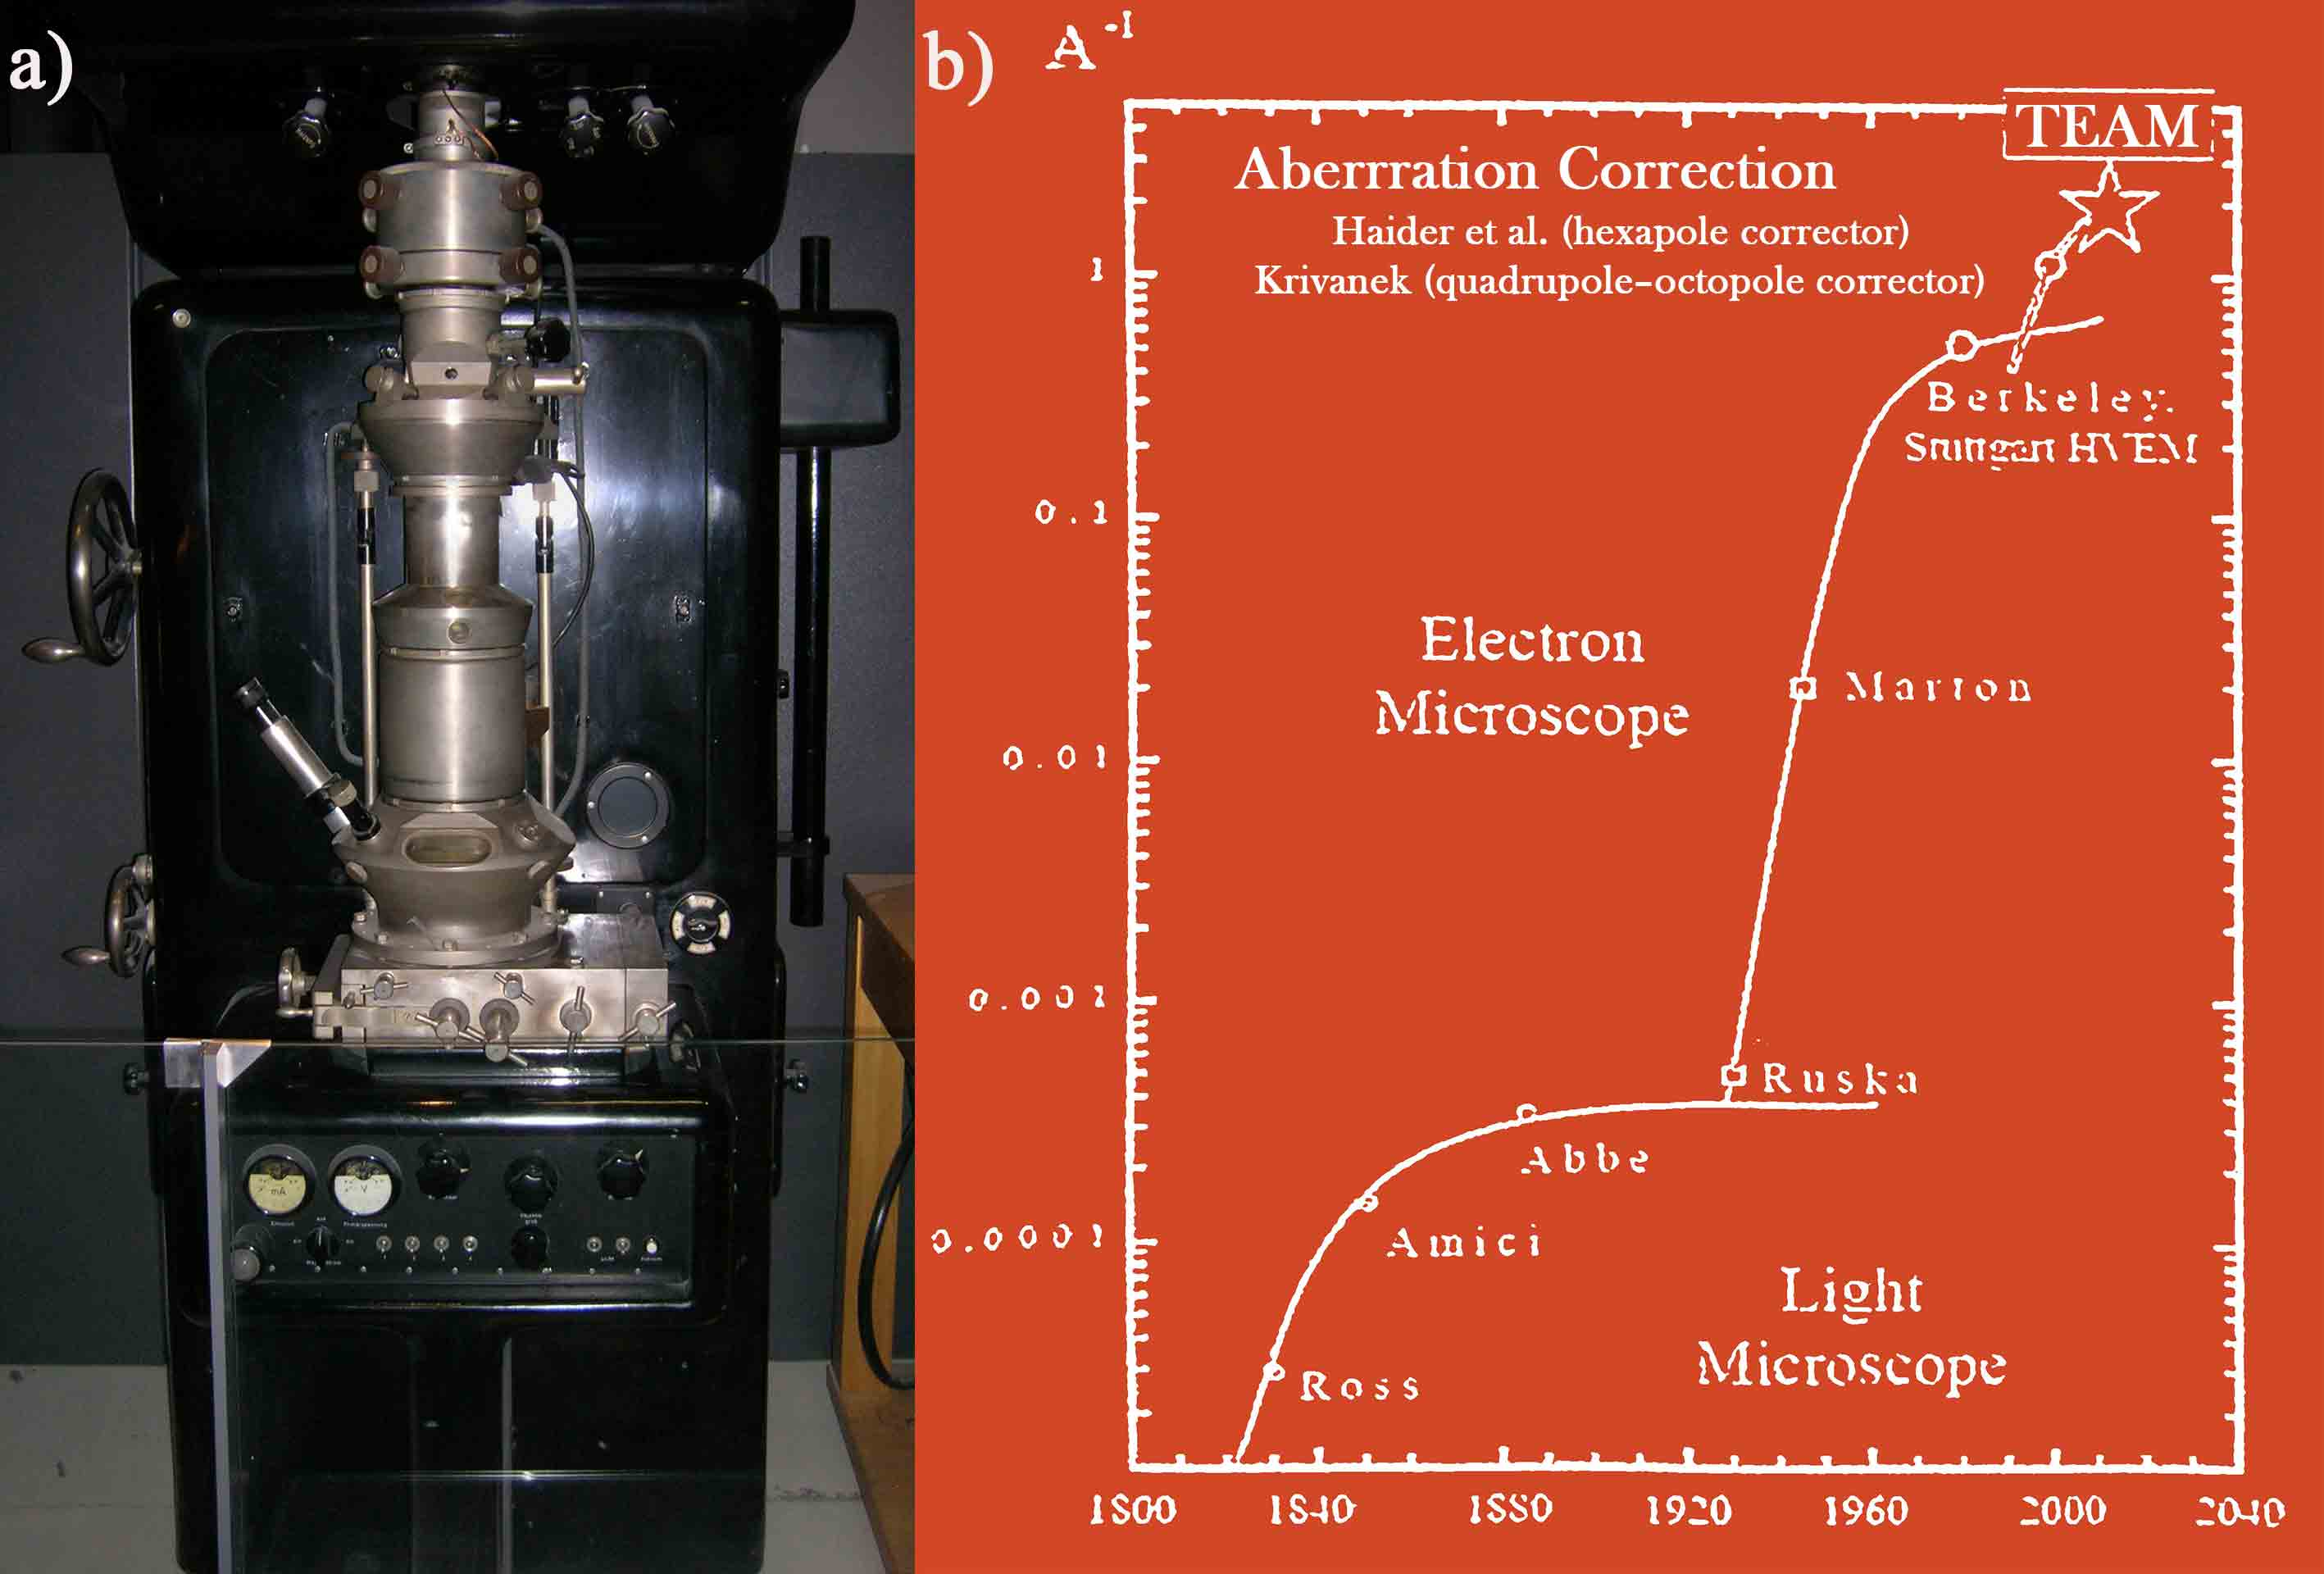
\includegraphics[width=0.8\textwidth]{../1.1/11}
	\caption{世界上第一台电子显微镜与显微镜分辨率发展曲线}\label{fig:11}
	\song\tuzhu{a) 世界上第一台电子显微镜;b) 显微镜分辨率发展曲线}
\end{figure}

材料的三维结构对其宏观性能具有非常重要的影响。比如铝合金中的析出相的形貌、尺寸以及分布决定其析出强化的效果;纳米颗粒的形貌和尺寸会影响其催化性能、分布状况等。揭示材料的三维结构、成分、分布等性质是材料科学研究中一个极其重要的问题。一般情况下,一张 TEM 照片只能揭示材料在某一平面上的结构与性质,获取材料的三维信息需要进行更复杂的实验与理论分析。三维电子断层成像~\cite{Frank2006,VanAarle2015,Heidari2013,Koning2013,Fakron2015}(three-dimensional electron tomography,3DET)技术是 TEM 中应用最广泛的三维重构技术,它利用物体多个方向的投影来恢复出物体内部的三维信息。3DET 起初被应用于生物科学的研究中,利用 TEM 的明场(bright field,BF)模式拍摄细胞或蛋白质在不同方向的投影以重构它们的三维结构~\cite{Baumeister1999,McEwen2001, McIntosh2001}。扫描透射电子显微镜(scanning transmission electron microscopy,STEM)以及高角环形暗场(high angle annular dark field,HAADF)成像模式可以获得与材料中原子质量呈线性关系的 $Z$ 衬度图像~\cite{Nellist2000}。它使得 TEM 可以拍摄到晶体材料的质厚投影图像,该技术的出现普及了 3DET 技术的应用~\cite{Kubel2005,Zhong2017,Alania2017,Lefebvre2015},并使其能够达到原子分辨率~\cite{Zhou2019,Chen2013,Miao2016,Zhu2013,Xu2015,Scott2012,WangCY2020}。由于 3DET 的实现需要收集大量的实验投影图像,它的实际重构精度受诸多因素的影响,如缺失锥~\cite{Persson2001,Lu2010,Aganj2007,Paavolainen2014,Yau1996,Trampert2016,Kovacik2014,Kupsch2015}、辐照损伤~\cite{Lee2008}、样品漂移~\cite{Ress1999,Jones2013,Diez2006,Printemps2016}等。这些问题在一般的 3DET 实验和重构过程中难以避免,它们通常会降低重构的分辨率,甚至在重构结果中引入假象。精确乃至定量地重构材料的三维形貌仍然是一个具有挑战性的课题。并且,这些因素使得原子分辨率的 3DET 重构的实现异常困难。
为了突破传统 3DET 重构中的困难,最近,科学家们不约而同地提出了一些 TEM 中原子分辨率三维重构的新方法~\cite{ChenFR2017,ChenFR2016,Jia2014,VanDyck2012,VanAert2011}。这些方法通过结合电子显微学的理论知识来分析少量、甚至单张 (S)TEM 原子像,以重构出材料内部的三维信息。由于使用的实验数据少,这样的三维重构方法受实验条件的限制减少,可操作性提高。这些新方法的理论的完善与应用的普及,将继续推动 TEM 中三维重构技术的发展。


\section{TEM 及其成像理论}
\subsection{TEM 发展简介}
1928 年,柏林科技大学的高压电及电气教授 Adolf Matthias 让 Max Knoll 领导一个研究小组以改进阴极射线示波器。这个研究小组由几个博士生组成,这些博士生包括 Ernst Ruska 和 Bodo von Borries。这组研究人员考虑了透镜设计和示波器的阵列排列,试图通过这种方式来找到更好的示波器设计方案,同时研制可以用于产生低放大倍数(接近 1:1)的电子光学原件。1931 年,这个研究组成功获得了在阳极光圈上放置的网格的电子放大图像。这个设备使用了两个磁透镜来达到更高的放大倍数,因此被称为世界上第一台电子显微镜~\cite{Knoll1932}(图 1.1a)。在同一年,西门子公司的研究室主任 Reinhold Rudenberg 提出了电子显微镜的静电透镜的专利~\cite{RudenbergReinhold1931}。

1927 年,Louis de Broglie 发表的论文中揭示了电子这种本认为是带有电荷的物质粒子的波动特性。电子波长可以通过徳布罗意公式根据电子的动能得出。由于在 TEM 中,电子的速度接近光速,需要对其进行相对论修正:
\begin{equation}
\lambda_e \approx \frac{h}{\sqrt{2m_0E(1+\frac{E}{2m_0c^2})}}
\end{equation}
其中,$h$ 表示普朗克常数,$m_0$ 表示电子的静质量,$E$ 是加速后的电子的能量,$c$ 是光速。TEM 研究组直到 1932 年才知道了这篇论文,随后,他们迅速的意识到了电子波的波长比光波波长小了若干数量级,理论上允许人们观察原子尺度的物质。

1938 年,Manfred von Ardenne 在西门子公司研发了世界上第一台 STEM。20 世纪 70 年代,芝加哥大学的 Albert Crewe 发明了场发射电子枪~\cite{Crewe1969},同时添加了高性能的物镜从而发明了现代的 STEM。这种设计可以通过环形暗场(annular dark field,ADF)成像技术对原子进行成像。到 20 世纪 80 年代末,90 年代初,STEM 的分辨率达到了 2 Å,这意味着材料的原子结构可以被清楚地观测。

1997 年,Max Haider 发明了世界上第一个球差矫正器~\cite{Haider1997},迎来了 TEM 分辨率提升的新纪元。2008 年,美国伯克利大学的 TEAM 项目(Transmission Electron Aberration-corrected Microscope Project)研发的球差矫正的 STEM 分辨率达到了 0.5 Å~\cite{Kisielowski2008}。2016 年得益于球差与色差双矫正器的运用,SALVE 项目(Sub-Angstrom Low-Voltage Electron Microscopy Project)研发的 TEM 在低加速电压下(20  keV)也能达到 1.4 Å 的分辨率~\cite{Linck2016}。

\subsection{TEM 的结构}
TEM 是以波长极短的电子束作为照明源,用电磁透镜聚焦成像的一种高分辨率高放大倍数的电子光学仪器。其电子光学系统构造如图 1.2 所示,分为照明系统、成像系统和观察记录系统。

照明系统由电子枪、聚光镜和相应的平移对中、倾斜调节装置组成。电子枪是一个由钨丝或六硼化镧制成的电子发射源~\cite{Buckingham1865}。通过将电子枪与高电压源相连,在电流足够大的时候,电子枪通过热电子发射或者场电子发射机制将电子发射入真空。

成像系统主要由物镜、中间镜和投影镜组成。物镜是用来形成第一幅高分辨电子显微图像~\cite{Garbrecht2011, DeBeeck1996}或电子衍射花样~\cite{Lynch1971, Wang1991,Wang1995,Spence1998,Cowley1968,Howie1961,Chen1995}的透镜。在电镜操作过程中,主要是利用中间镜的可变倍率来控制电镜的总放大倍数。如果把中间镜的物平面和物镜的像平面重合,则在荧光屏上得到一幅放大像,这就是 TEM 中的成像操作;如果把中间镜的物平面和物镜的背焦面重合,则在荧光屏上得到一幅电子衍射花样,这就是 TEM 中的电子衍射操作。投影镜的作用是把经中间镜放大的像进一步放大,并投影到荧光屏上。

TEM 的观察记录系统包括荧光屏,基于胶片或者基于电荷耦合器件(charge coupled device,CCD)的图像记录系统。

\begin{figure}[htbp]
	\vspace{\baselineskip}
	\centering
	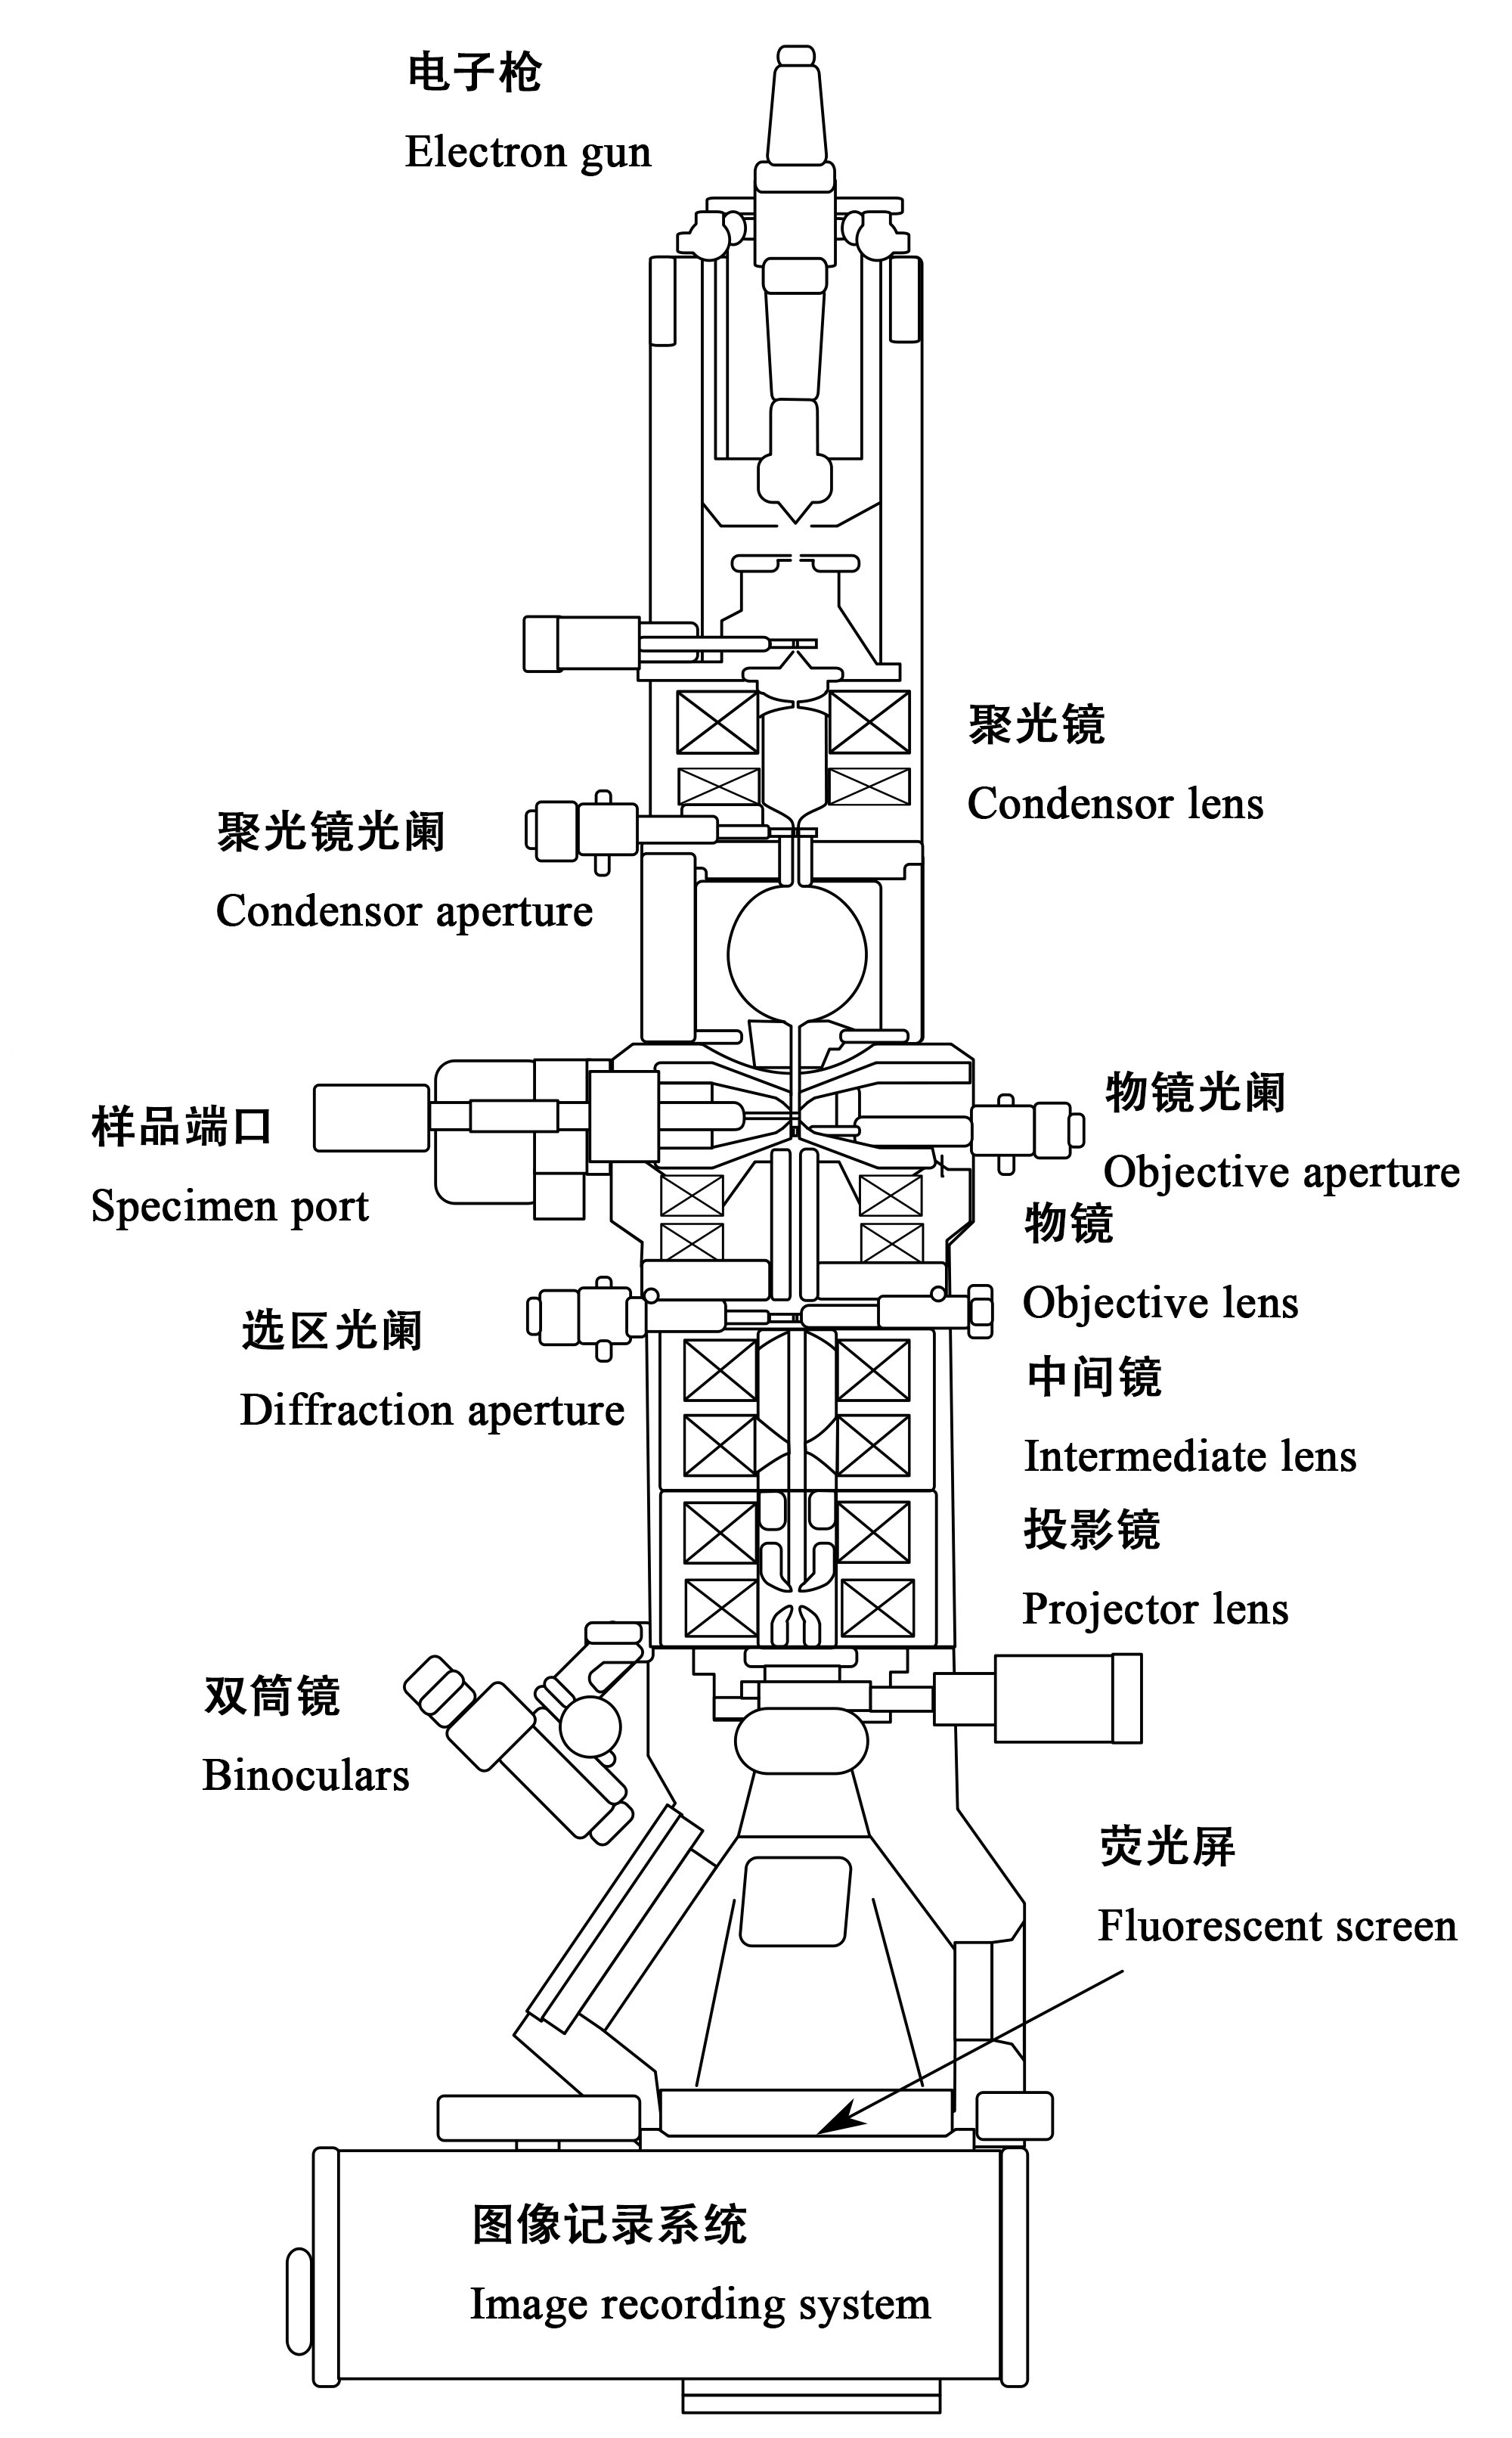
\includegraphics[width=0.9\textwidth]{../1.2/12}
	\caption{透射电镜结构示意图}\label{fig:12}
\end{figure}

\subsection{(S)TEM 成像原理}
如图 1.3a 所示,在 TEM 模式中,电子束在聚光镜的调制下,以平行束的形式 ($\psi_{in} (\boldsymbol{r})=1$)入射到样品表面。一般,透射电镜的样品厚度小于 100 nm,电子束与样品作用之后可以穿过样品,从而携带了样品的内部结构信息。出射波函数 $\psi_{out} (\boldsymbol{r})$ 经物镜聚焦后形成图像 $I_D$,图像经中间镜和投影镜放大、投射到图像记录系统~\cite{Gomez2010}:
\begin{equation}I_{D}(\boldsymbol{r})=\left|\psi_{D}(\boldsymbol{r})\right|^{2}\end{equation}
\begin{equation}\psi_{D}(\boldsymbol{r})=\mathcal{F}^{-1}\left\{\mathcal{F}\left\{\psi_{\text {out}}(\boldsymbol{r})\right\} \textit{CTF}(\boldsymbol{k})\right\}\end{equation}
其中,$\boldsymbol{r}$ 和 $\boldsymbol{k}$ 是实空间和倒空间的二维平面矢量,$\mathcal{F}$ 和 $\mathcal{F}^{-1}$ 表示二维傅里叶变换与逆变换,$\textit{CTF}$ 是衬度传递函数(contrast transfer function,CTF):
\begin{equation}\textit{CTF} (\boldsymbol{k})=\exp \{-i \chi(\boldsymbol{k})\} E_{\delta}(\boldsymbol{k}) E_{\alpha}(\boldsymbol{k})\end{equation}
$\chi(\boldsymbol{k})$ 是电磁透镜的像差引起的相位变化,它描述了电子波偏离平面波的程度,它以极角 $\theta$ 和方位角 $\phi$ 的展开式为:
\begin{equation}\chi(\theta, \phi)=\frac{2 \pi}{\lambda} \sum_{m n} \frac{\theta^{n+1}}{n+1}\left[C_{n m a} \cos (m \phi)+C_{n m b} \sin (m \phi)\right]\end{equation}
其中 $\lambda$ 是电子波长,$n$ 和 $m$ 是非负整数,代表了像差的阶数,$C_{nma}$ 和 $C_{nmb}$ 是各阶像差系数,例如 $C_{10}$ 是欠焦量、$C_{30}$ 是三级球差,具体可参考 Kirkland 的文献~\cite{Kirkland2011}。极角 $\theta$ 和方位角 $\phi$ 与倒空间坐标 $\boldsymbol{k}$ 具有如下换算关系:
\begin{equation}\theta=\lambda k\end{equation}
\begin{equation}\phi=\left\{ \begin{array}{r}
\textnormal{-}\arctan \left(\frac{k_{y}}{k_{x}}\right), \mid k_{x} \neq 0, k_{y}<0 \\
\arctan \left(\frac{k_{y}}{k_{x}}\right), \mid k_{x} \neq 0, k_{y} \geq 0 \\
\textnormal{-}\pi, \mid k_{x}=0, k_{y}<0 \\
\pi, \mid k_{x}=0, k_{y} \geq 0
\end{array} \right. \end{equation}
$E_{\delta}(k)$ 和 $E_{\alpha}(k)$ 分别是时间和空间相干性引起的衰减包络函数~\cite{Chen2004,Chang2006}:
\begin{equation}E_{\delta}(\boldsymbol{k})=\exp \left\{-\frac{1}{2}(\pi \lambda \delta)^{2} k^{2}\right\}\end{equation}
\begin{equation}E_{\alpha}(\boldsymbol{k})=\exp \left\{-\left(\frac{\pi \alpha}{\lambda}\right)^{2}\left[C_{30} \lambda^{3} k^{3}-C_{10} \lambda k\right]^{2}\right\}\end{equation}
其中 $\alpha$ 是电子束的会聚半角,$\delta$ 是焦点扩展度,它描述了物镜电流电压的稳定性以及电子枪的能量扩展度:
\begin{equation}\delta=C_{c}\left[4\left(\frac{\Delta I}{I}\right)^{2}+\left(\frac{\Delta E}{E}\right)^{2}+\left(\frac{\Delta V}{V}\right)^{2}\right]^{1 / 2}\end{equation}
其中 $C_c$ 是物镜的色差系数。

在 STEM 成像模式中,电子束由聚光镜聚焦成一个极小的束斑,而后在水平面上对样品进行扫描,生成一幅扫描图像。电子束斑的表达式为~\cite{Xin2009}:
\begin{equation}
\psi_{in}(\boldsymbol{r})=A_r\mathcal{F}\left\{H(k)\textit{CTF}(\boldsymbol{k})\right\}
\end{equation}
其中 $A_r$ 是归一化因子,仅与 $\alpha/\lambda$ 有关,$H$ 是光阑函数,在 $k\leq\alpha/\lambda$ 时为 1,$k>\alpha/\lambda$ 时为 0。

电子束穿过样品后,携带了束斑所在位置的样品的内部结构信息,经背焦面上的环形探测器收集,形成 STEM 信号~\cite{Bosch2015}。如图 1.3b 所示,根据探测器的尺寸和位置不同,所形成的信号可以分为 BF、环形明场~\cite{Ma2018,Gao2017,Kim2017,Findlay2010}(annual bright field,ABF),ADF~\cite{Kirkland2011,Xin2009,Hillyard1993,Hillyard1995,Loane1992},HAADF。HAADF 信号由电子与样品原子核之间的卢瑟福散射形成~\cite{VandenBroek2012},一般认为其与样品中原子的原子序数 $Z^{\sim 1.7}$ 在一级近似下呈正比~\cite{Nellist2000,Midgley2003,Wang1991-1,Treacy1993},所以 HAADF-STEM 图像被认为是样品的质厚衬度~\cite{Kubel2005}。通过分析透射电子的能量损失谱~\cite{Batson1993,Fink1984,Kimoto2007}(electron energy loss spectroscopy,EELS),STEM 还可以分析材料的元素成分信息。
\begin{figure}[htbp]
	\vspace{\baselineskip}
	\centering
	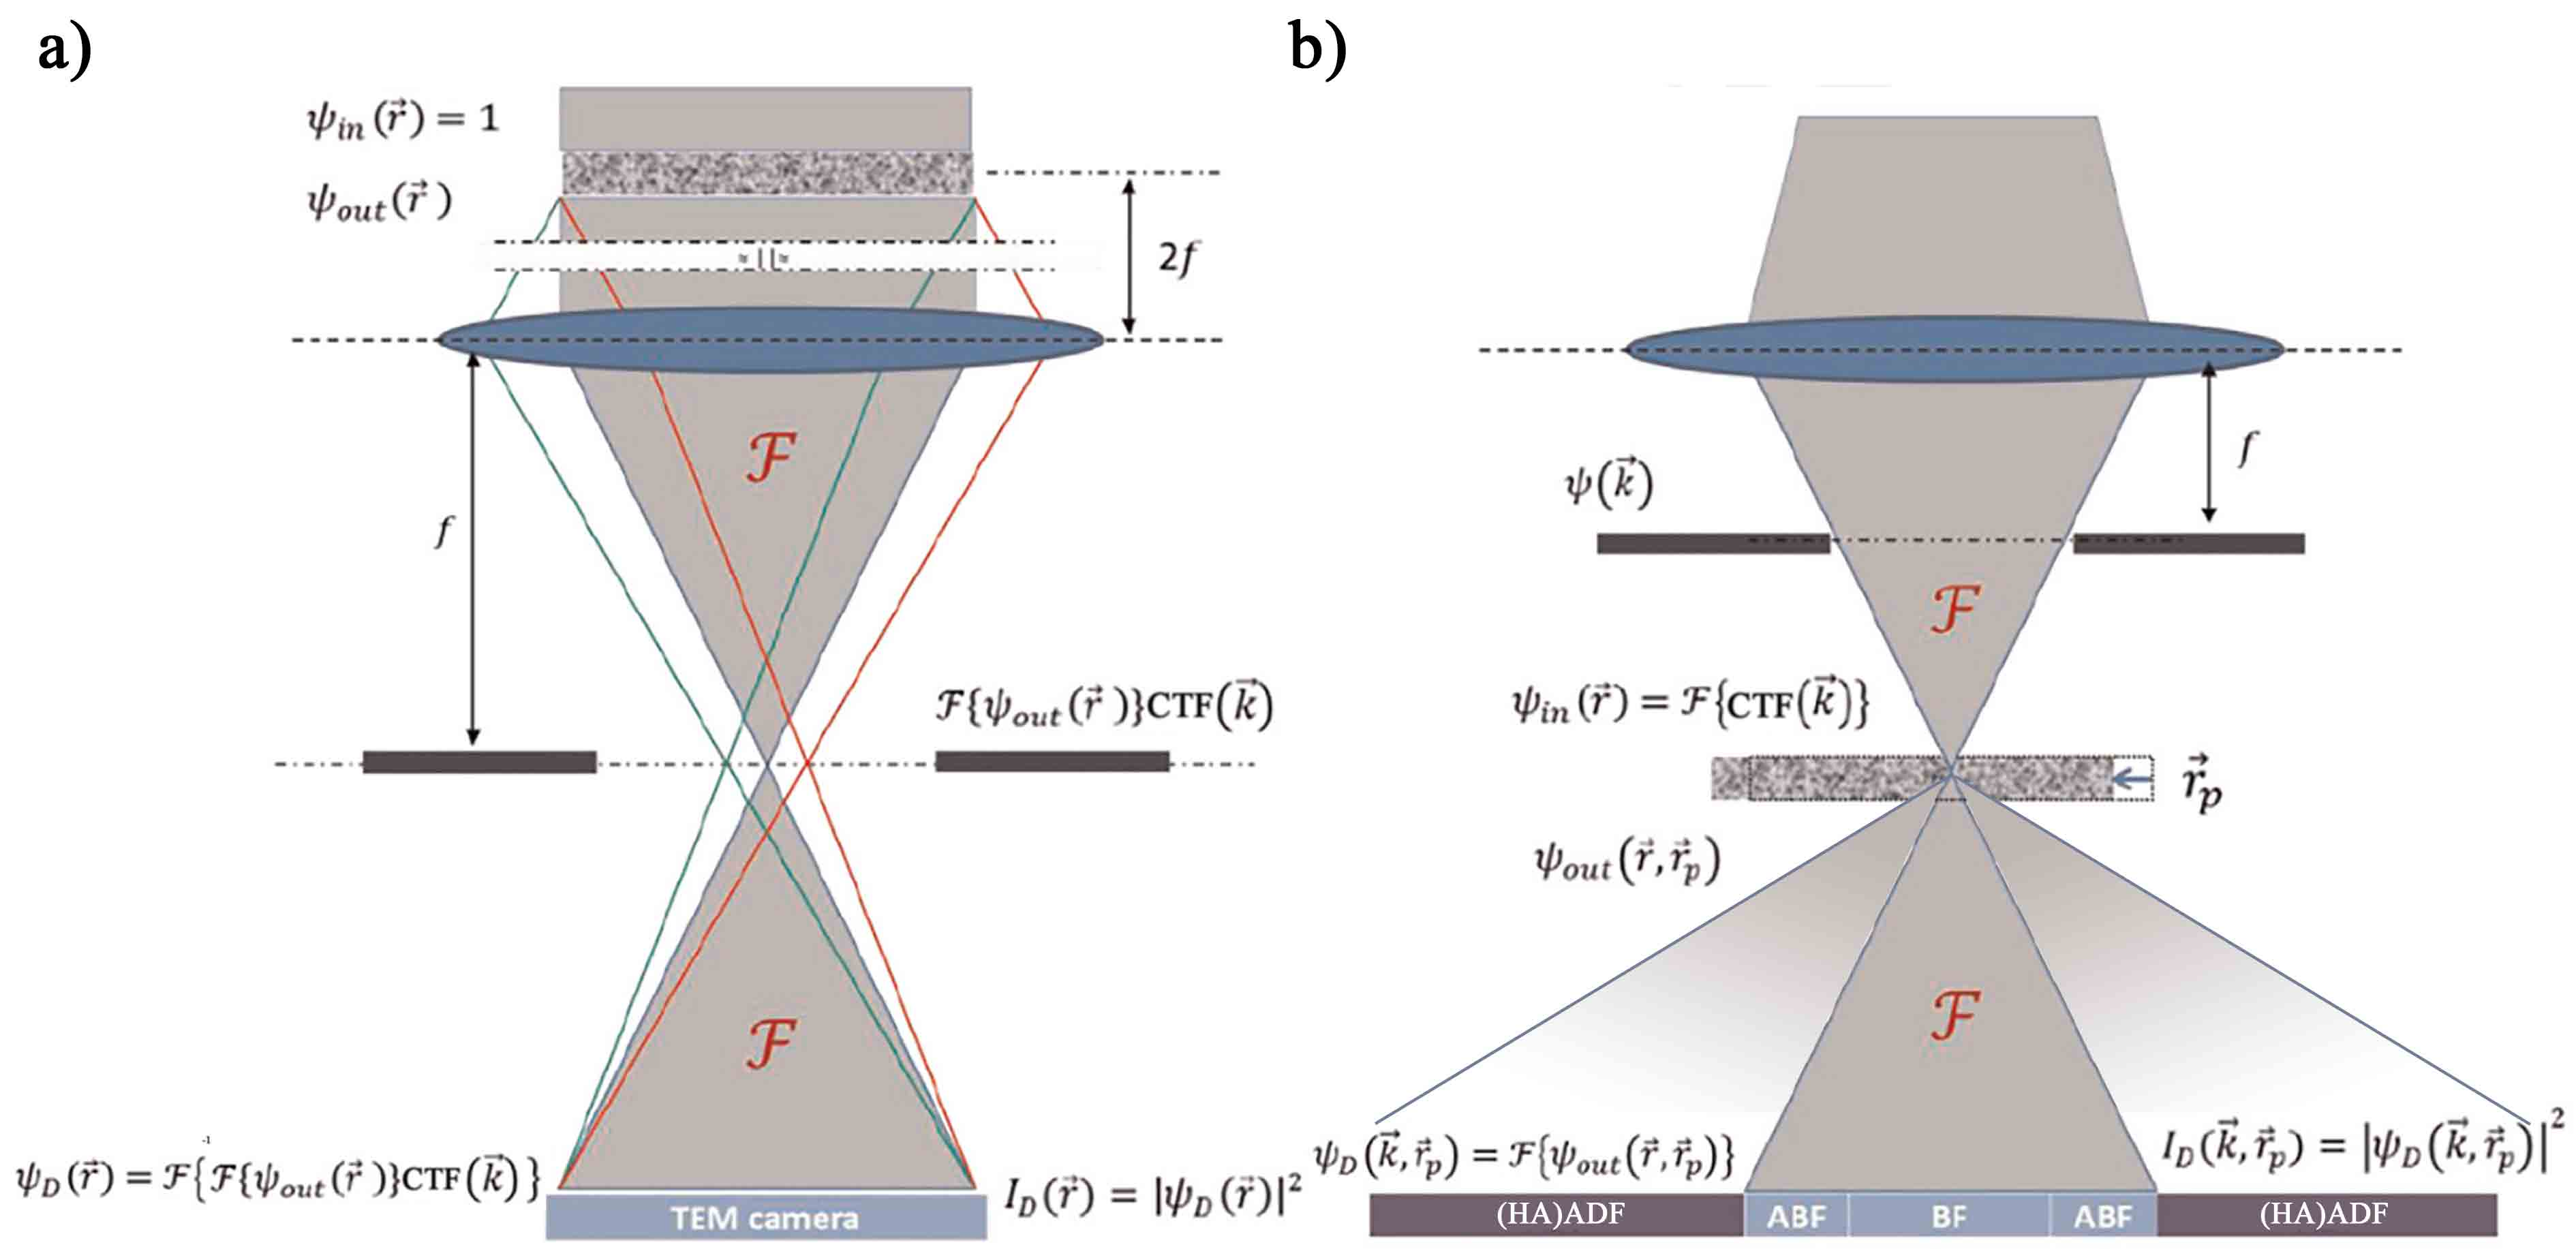
\includegraphics[width=0.95\textwidth]{../1.3/13}
	\caption{(S)TEM 光路示意图$^{[59]}$}\label{fig:13}
	\song\tuzhu{a) TEM 光路示意图;b) STEM 光路示意图}
\end{figure}

\subsection{多片层法像模拟}
\subsubsection{传统多片层法}
1957 年,J.M. Cowley 和 A.F. Moodie 基于物理光学原理提出多片层法~\cite{Cowley1957}(multislice),为模拟电子束在物体中的多重弹性散射提供了有效的手段。在随后的几十年内,高分辨像的数值模拟方法发展迅速并日趋成熟,多片层法已被广泛使用于各类材料的 TEM 图像分析之中~\cite{Cai2009,Cai2012,Chen1997,Ming2013,Chen1996}。

如图 1.4 所示,多片层法主要分为以下 5 个步骤:

(1)把物体沿垂直于电子束入射方向分割成许多厚度为 $\Delta z$ 的薄层。

(2)在每一个片层内,将其中的静电势投影到上表面。晶体中的静电势的表达式为:
\begin{equation}\varphi(\boldsymbol{r})=\frac{\lambda}{\delta \Omega} \sum_{\boldsymbol{k}} F(\boldsymbol{k}) \exp [-2 \pi i(\boldsymbol{k} \cdot \boldsymbol{r})]\end{equation}
其中 $\lambda$ 是电子波长,$\Omega$ 是单胞体积,$\delta$ 是交互作用因子,$F$ 是晶体结构因子。

(3)由于每一个片层厚度很小,可以利用相位物体近似~\cite{cai2004,Ming2017},将投影势场看作相位光栅 $q$,电子与其作用时只改变相位,不改变振幅:
\begin{equation}
q(\boldsymbol{r})=\exp\left(i\sigma\int\phi(\boldsymbol{r},z)dz\right)
\end{equation}
其中 $\sigma$ 是相互作用常数。

(4)电子在片层内的真空中传播用菲涅尔传播函数表示:
\begin{equation}
p(\boldsymbol{r})=\frac{1}{i\Delta z \lambda}\exp\left(-\frac{ik\boldsymbol{r}^2}{2\Delta z}\right)
\end{equation}

(5)如此,电子在整个实空间中的传播的表达式为:
\begin{equation}\psi(\boldsymbol{r})=q_{n}(\boldsymbol{r}) \cdot\left[\cdots\left[q_{2}(\boldsymbol{r}) \cdot\left[q_{1}(\boldsymbol{r}) \otimes p_{1}(\boldsymbol{r})\right] \otimes p_{2}(\boldsymbol{r})\right] \cdot \cdot\right] \otimes p_{n}(\boldsymbol{r})\end{equation}
多片层法中的卷积运算可以通过傅里叶变换转换为标量积运算,大大减小运算量。所以传统的多片层法是在倒空间中进行计算的。
\begin{figure}[htbp]
	\vspace{\baselineskip}
	\centering
	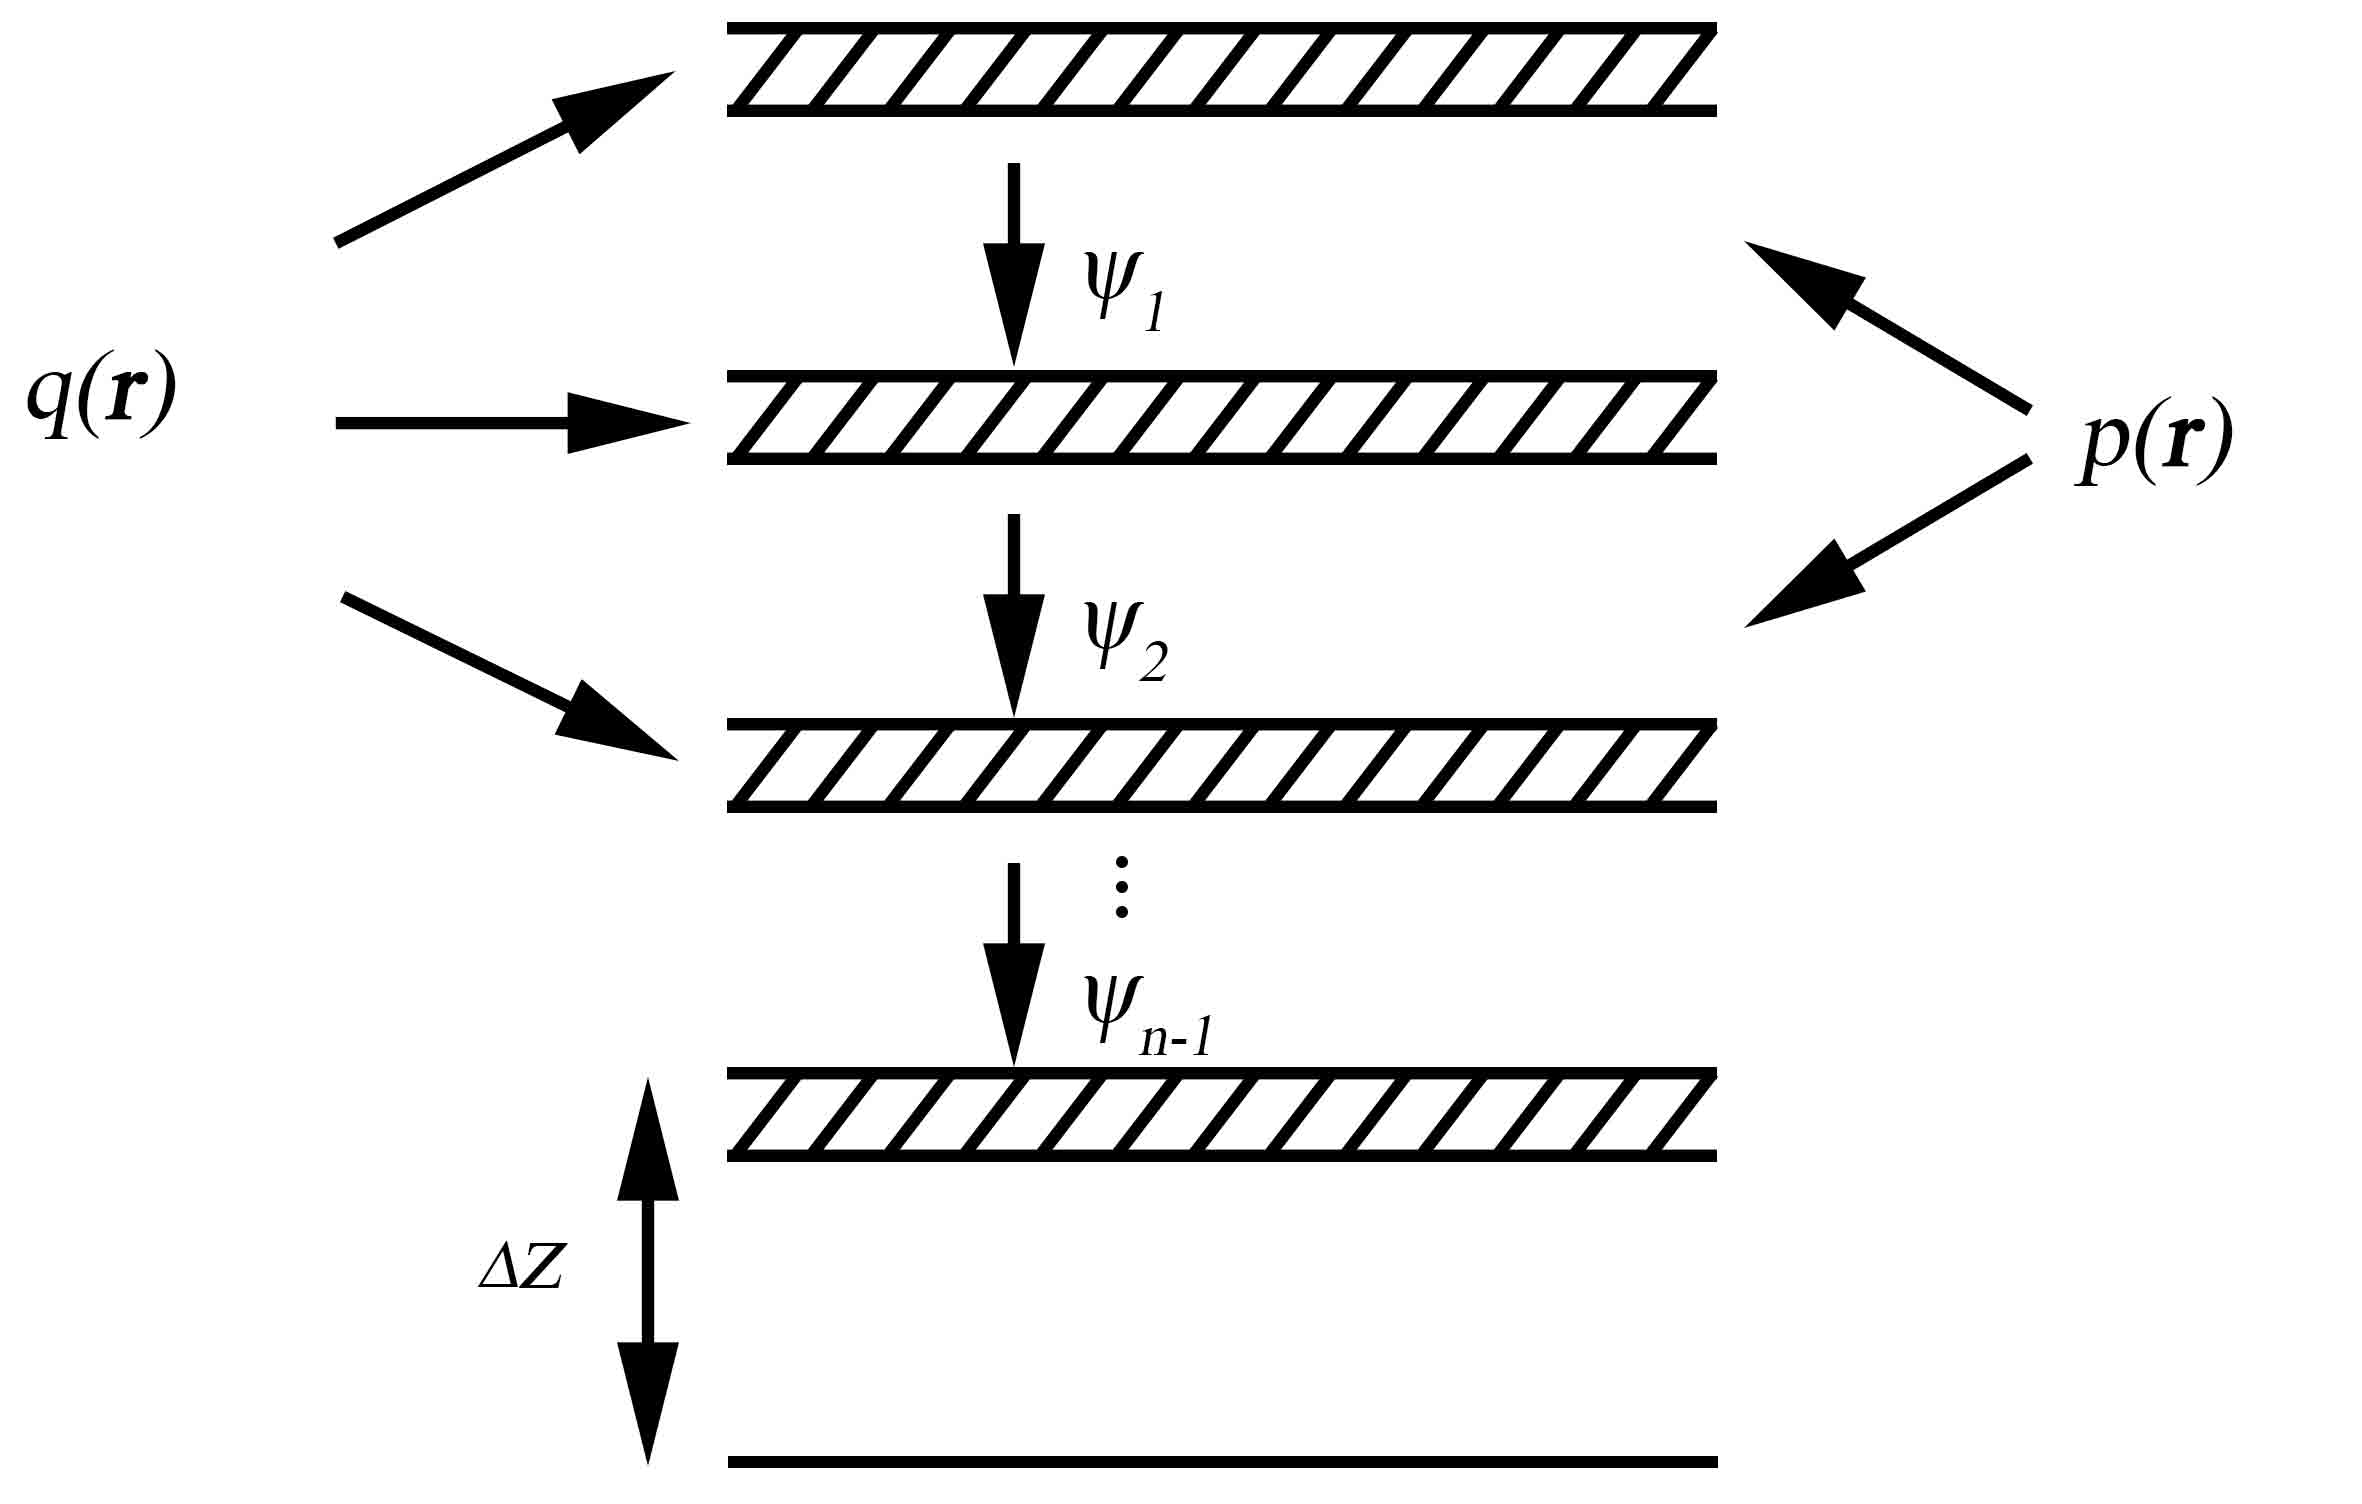
\includegraphics[width=0.6\textwidth]{../1.4/14}
	\caption{多片层法中,各片层中透射函数和传播函数的示意图}\label{fig:14}
\end{figure}
\subsubsection{实空间多片层法}
1980 年,D. Van Dyck 基于量子力学求解薛定谔方程,提出了一种在实空间中进行计算的多片层法~\cite{VanDyck1980}。该方法通过片层分割的方式,在高能近似下求解定态薛定谔方程来计算电子波函数~\cite{Coene1984,VanDyck1984,Coene1984-1},以下是高能近似修正的定态薛定谔方程:
\begin{equation}
\frac{\partial \psi (\boldsymbol{R})}{\partial z} = \left[ \frac{i\lambda}{4\pi}\triangle + i\sigma V(\boldsymbol{R}) \right] \psi (\boldsymbol{R}) 
\end{equation}
其中 $\psi (\boldsymbol{R})$ 是三维电子波函数,$\lambda$ 和 $\sigma$ 分别为电子波波长和相互作用常数,$V(\boldsymbol{R})$ 是晶体的静电势,$\triangle$ 是二维拉普拉斯算符。

求解该微分方程,可以使用如图 1.4 所示的方式,将晶体势场沿 $z$ 方向分割成许多厚度为 $\Delta z$ 的薄层,于是出射面波函数与入射面波函数之间的关系可以表达为~\cite{Chen1996}:
\begin{equation}
\psi_n (\boldsymbol{r}) = \hat{A}_n \hat{A}_{n-1} \cdots \hat{A}_1 \psi_0(\boldsymbol{r})
\end{equation}
其中 $\hat{A}_n$ 是严格的电子波函数在片层之间的传播运算符:
\begin{equation}\begin{aligned}
&\hat{A}_{n}(\boldsymbol{r})=1+\int_{(n-1) \Delta z}^{n \Delta z}\left[\frac{i \lambda \Delta}{4 \pi}+i \sigma V(\boldsymbol{r}, z_1)\right] d z_1+\cdots+\int_{(n-1) \Delta z}^{n \Delta z}\left[\frac{i \lambda \Delta}{4 \pi}+\right.\\
&i \sigma V\left(\boldsymbol{r}, z_{1}\right)\Bigg] d z_{1} \int_{(n-1) \Delta z}^{z_{1}} \ldots \int_{(n-1) \Delta z}^{z_{k}-1}\left[\frac{i \lambda \Delta}{4 \pi}+i \sigma V\left(\boldsymbol{r}, z_{k}\right)\right] d z_{k}+\cdots 
\end{aligned}\end{equation}
当 $\Delta z$ 非常小时,片层内沿 $z$ 方向的势场变化可以忽略不计,则 $\hat{A}_n$ 可以被简化为 $\hat{B}_n$:
\begin{equation}
\hat{B}_n (\boldsymbol{r}) = \exp\left[i\Delta z \left( \frac{\lambda \triangle}{4\pi} + \sigma V_n^P (\boldsymbol{r}) \right)\right]
\end{equation}
其中 $V_n^P (\boldsymbol{r})$ 是第 n 片层中的平均静电势。根据 Baker–Campbell–Hausdorff 公式,$\hat{B}_n (\boldsymbol{r})$ 的 Zassenhaus 展开的一级近似为:
\begin{equation}
\hat{M}_n (\boldsymbol{r}) = \exp \left(i\Delta z \frac{\lambda \triangle}{4\pi}\right) \cdot \exp \left(i \Delta z \sigma V_n^P(\boldsymbol{r})\right)
\end{equation}
于是:
\begin{equation}
\psi_n(\boldsymbol{r}) = \hat{M}_n \hat{M}_{n-1} \cdots \hat{M}_1 \psi_0(\boldsymbol{r})
\end{equation}
公式(1.21)和传统的多片层法公式(1.15)是完全一致的。

以上是求解高能近似下的薛定谔方程的结果。J.H. Chen 和 D. Van Dyck 等在 1997 年提出了薛定谔方程的精确解法~\cite{Chen1997},C.Y. Cai,W.Q. Ming 和 J.H. Chen 等后来实现了该方法的数值计算应用,将其命名为全修正多片层法,并证明了它在低能电子动力学衍射模拟中的必要性~\cite{Cai2009,Ming2013,MWQ2018}。

\subsubsection{环绕效应}
在模拟计算中,由于电子波函数的调制和传递常常在倒空间中进行计算,所以傅里叶变换被频繁地使用于波函数在实空间与倒空间之间的变换。由于离散傅里叶变换(快速傅里叶变换)隐含的周期性,在实际运算过程中波函数在一个无穷大的周期性阵列中重复。这种周期性假设会使波函数的左右、上下边界相互环绕,产生计算误差,因此被称为环绕效应~\cite{Kirkland2010}(wrap around effect)。

如果样品超胞不具备周期性,模拟的边界处会引入显著的假象。如图 1.5 所示,在一个从上至下厚度梯度变化的超胞的模拟像中,下边界处出现了异常的深色衬度,这是上边界较厚的部分对下边界产生的环绕效应导致的计算误差。为了得到准确的计算结果,一般会在超胞周围增加缓冲区域或者真空。缓冲区域或真空的宽度应根据情况,通过测试来确定。消除环绕效应带来的误差,是图像定量分析的一个必要步骤。

\begin{figure}[htbp]
	\vspace{\baselineskip}
	\centering
	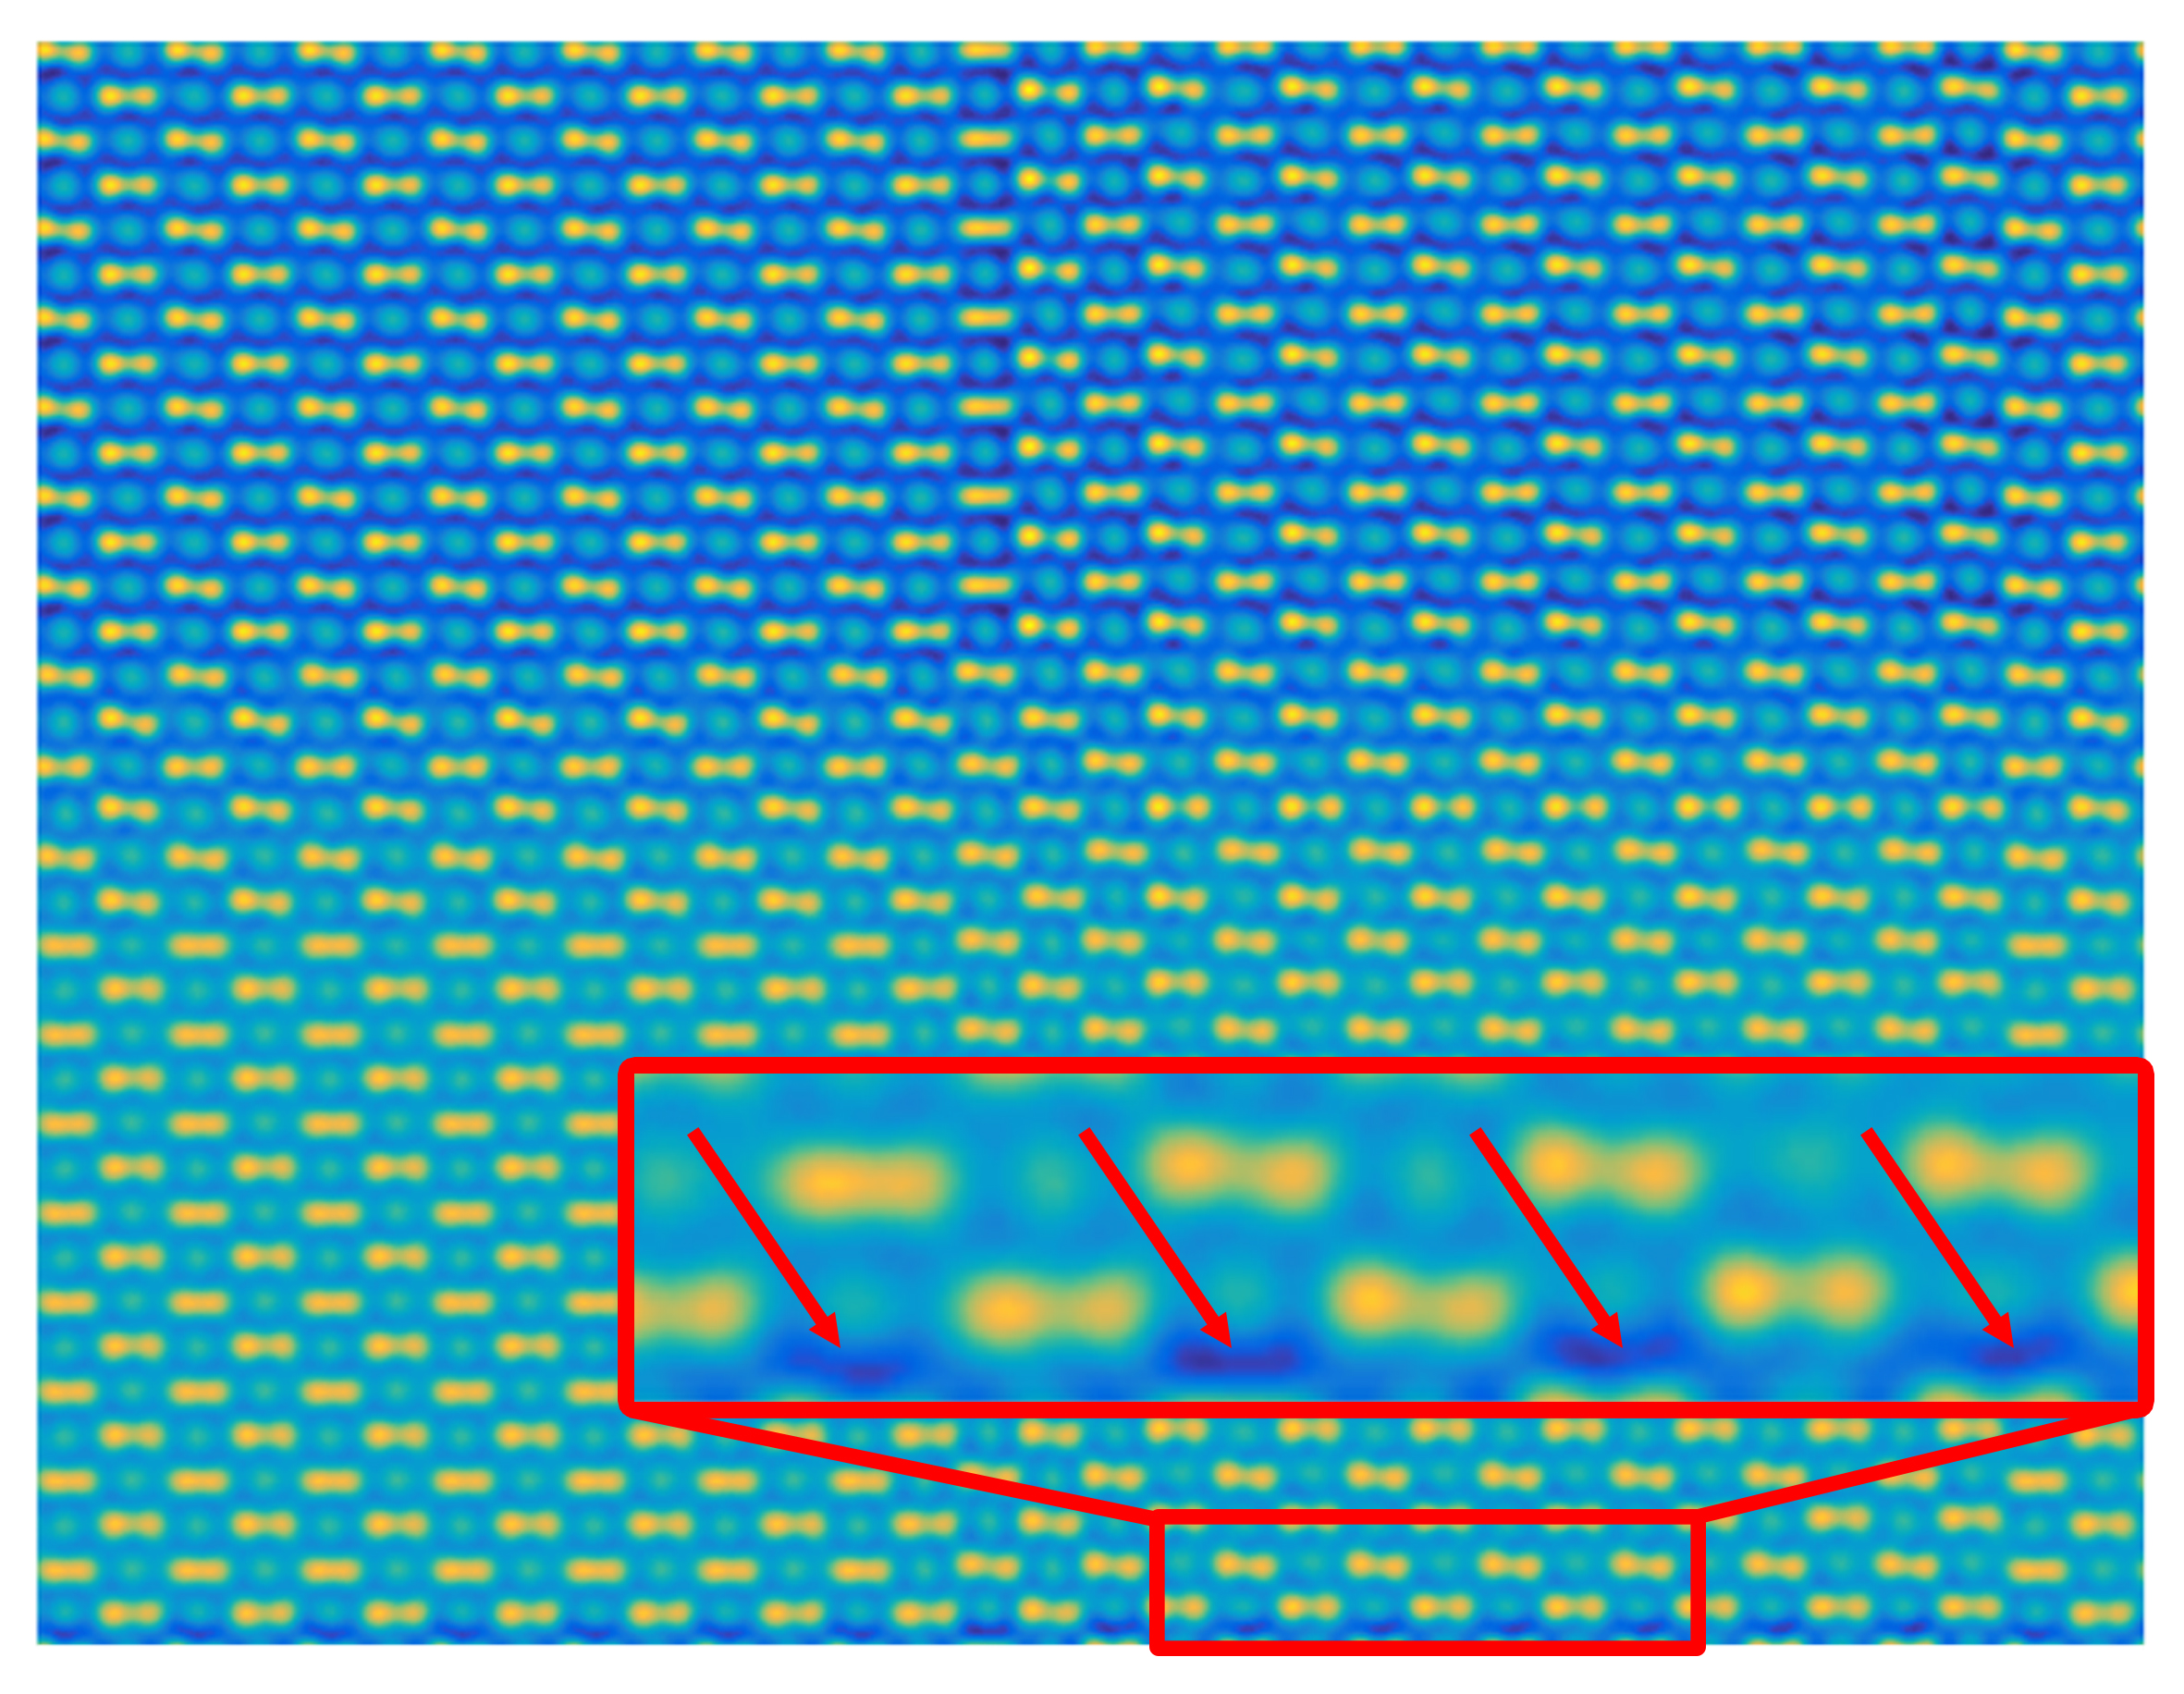
\includegraphics[width=0.6\textwidth]{../1.5/15}
	\caption{环绕效应示意图}\label{fig:15}
\end{figure}

\subsection{调制传递函数}

实验拍摄的 TEM 照片的衬度通常是理论模拟图像衬度的 3 倍以上。该现象最早由 M.J. Hÿtch 和 W.M. Stobbs~\cite{Hytch1994} 发现,这种图像衬度的比值被称为斯托布斯因子(Stobbs factor)。斯托布斯因子妨碍了对实验图像的定量分析。A. Thust~\cite{Thust2009} 指出,导致这种衬度差异的一个重要因素是像模拟时没有考虑 CCD 相机的调制传递函数(Modulation transfer function, MTF)对图像衬度的影响。

TEM 所成的像 $f$ 在经过 CCD 相机上的闪烁体时,会使 $f$ 卷积上一个旋转对称的点扩散函数,$\textit{psf}_{sc}$,然后才被相机记录。而在像素化的过程中,这个图像将进一步卷积上像素的形状函数 $\textit{psf}_{px}$,接着与一个梳齿函数 $c$ 相乘,最终记录的图像 $h$ 可表达为:
\begin{equation}
h=(f\otimes \textit{psf}_{sc} \otimes \textit{psf}_{px}) \cdot c
\end{equation}
其中 $\otimes$ 是卷积符号,$\cdot$ 是标量积符号。该式的傅里叶形式是:
\begin{equation}
H = (F \cdot \textit{MTF}_{sc}\cdot \textit{MTF}_{px})\otimes C
\end{equation}
其中 $H$,$F$,$\textit{MTF}_{sc}$,$\textit{MTF}_{px}$ 和 $C$ 分别是 $h$,$f$,$\textit{psf}_{sc}$,$\textit{psf}_{px}$,$c$ 的傅里叶变换。$\textit{MTF}_{sc}$ 是闪烁体的 MTF,在实际中需要测量。$\textit{MTF}_{px}$ 和 $C$ 可参考文献~\cite{VanBroek2012}。



\section{3DET 原理}
\subsection{概述}
3DET 的重构原理与计算机断层成像(computerized tomography,CT)技术相同。它的重构算法很多,主要分为变换法和代数法两类~\cite{Kak1988}。变换法是基于反拉登变换的数学解析方法,主要有滤波反投影(filtered back projection,FBP)和权重反投影~\cite{Liu2016,Cho1994}(weighted back projection,WBP)。代数法基于求解线性方程组的形式来实现图像重建,是数值求解法,主要包括代数重构技术~\cite{Gordon1970}(algebraic reconstruction technique,ART),同时迭代重构技术~\cite{Gregor2008,Okariz2017}(simultaneous iteration reconstruction technique,SIRT),同时代数重构技术~\cite{Jiang2003,Andersen1984}(simultaneous algebraic reconstruction technique,SART)等。另外,根据傅里叶中心切片定理~\cite{Garces2011,Bracewell1990}(Fourier central slice theorem)实现图像重建的过程需要解决数据在笛卡尔坐标和极坐标之间的转换,通常这类方法也是通过迭代的方式进行数值求解,如等斜率技术~\cite{Xu2015,Scott2012,Lee2008,Miao2005,Mao2010}(equally sloped technique,EST)。此外,由于 3DET 通常情况下是不适定问题,在重构算法中使用正则化或引入先验知识在某些情况下能够有效改善重构结果。最近,更有研究者利用深度学习技术引入大量先验知识来解决 3DET 中的难题。
3DET 在实际应用时,会遇到很多问题,比如缺失锥~\cite{Persson2001,Lu2010,Aganj2007,Paavolainen2014,Yau1996,Trampert2016,Kovacik2014,Kupsch2015}、辐照损伤~\cite{Lee2008}、样品漂移~\cite{Ress1999,Jones2013,Diez2006,Printemps2016}等。这些问题会限制重构分辨率甚至导致重构中出现假象。3DET 的分辨率还受采样和电镜分辨率等的限制~\cite{Hovden2014}。
\subsection{变换法}
\subsubsection{拉登变换}
拉登变换是函数在给定路径上的线积分,这里的函数表示研究对象的物理性质。拉登变换由 J. Radon 于 1917 年提出~\cite{Radon1917}。在 3DET 中,拉登变换的结果是未知物体 $f$ 的投影。由于一个偏心点的拉登变换形态上像一条正弦曲线,所以拉登变换得到的投影通常被称作 sinogram。
拉登变换的原理如下:
令 $f(\boldsymbol{r})=f(x, y)$ 是 $\mathbb{R}^2$ (二维实数集)上的紧支撑连续函数,拉登变换 $\mathcal{R}f$ 是定义在 $\mathbb{R}^2$ 中直线空间 $L$ 上的函数,沿每一条直线的线积分如下:
\begin{equation}
\mathcal{R}f(L) = \int _L f(\boldsymbol{r})|d\boldsymbol{r}|
\end{equation}
具体地,任何直线 $L$ 之于弧长 $l$ 都可被表达为:
\begin{equation}
\left( x,y \right) = \left( (l\sin\alpha + s \cos\alpha), (-l \cos\alpha + s \sin\alpha)\right)
\end{equation}
其中 $s$ 是直线 $L$ 到原点的距离,$\alpha$ 是直线 $L$ 的法向量与 $x$ 轴的夹角。于是,$(\alpha,s)$ 可被当作直线空间的坐标系的基矢量,拉登变换在此坐标系下表达为:
\begin{equation}
\mathcal{R}f(\alpha,s)= \int_{-\infty}^{\infty}f\left( x,y\right)dl = \int_{-\infty}^{\infty}f\left( (l \sin \alpha + s \cos\alpha),(-l \cos\alpha + s \sin\alpha)\right)dl
\end{equation}

\begin{figure}[htbp]
	\vspace{\baselineskip}
	\centering
	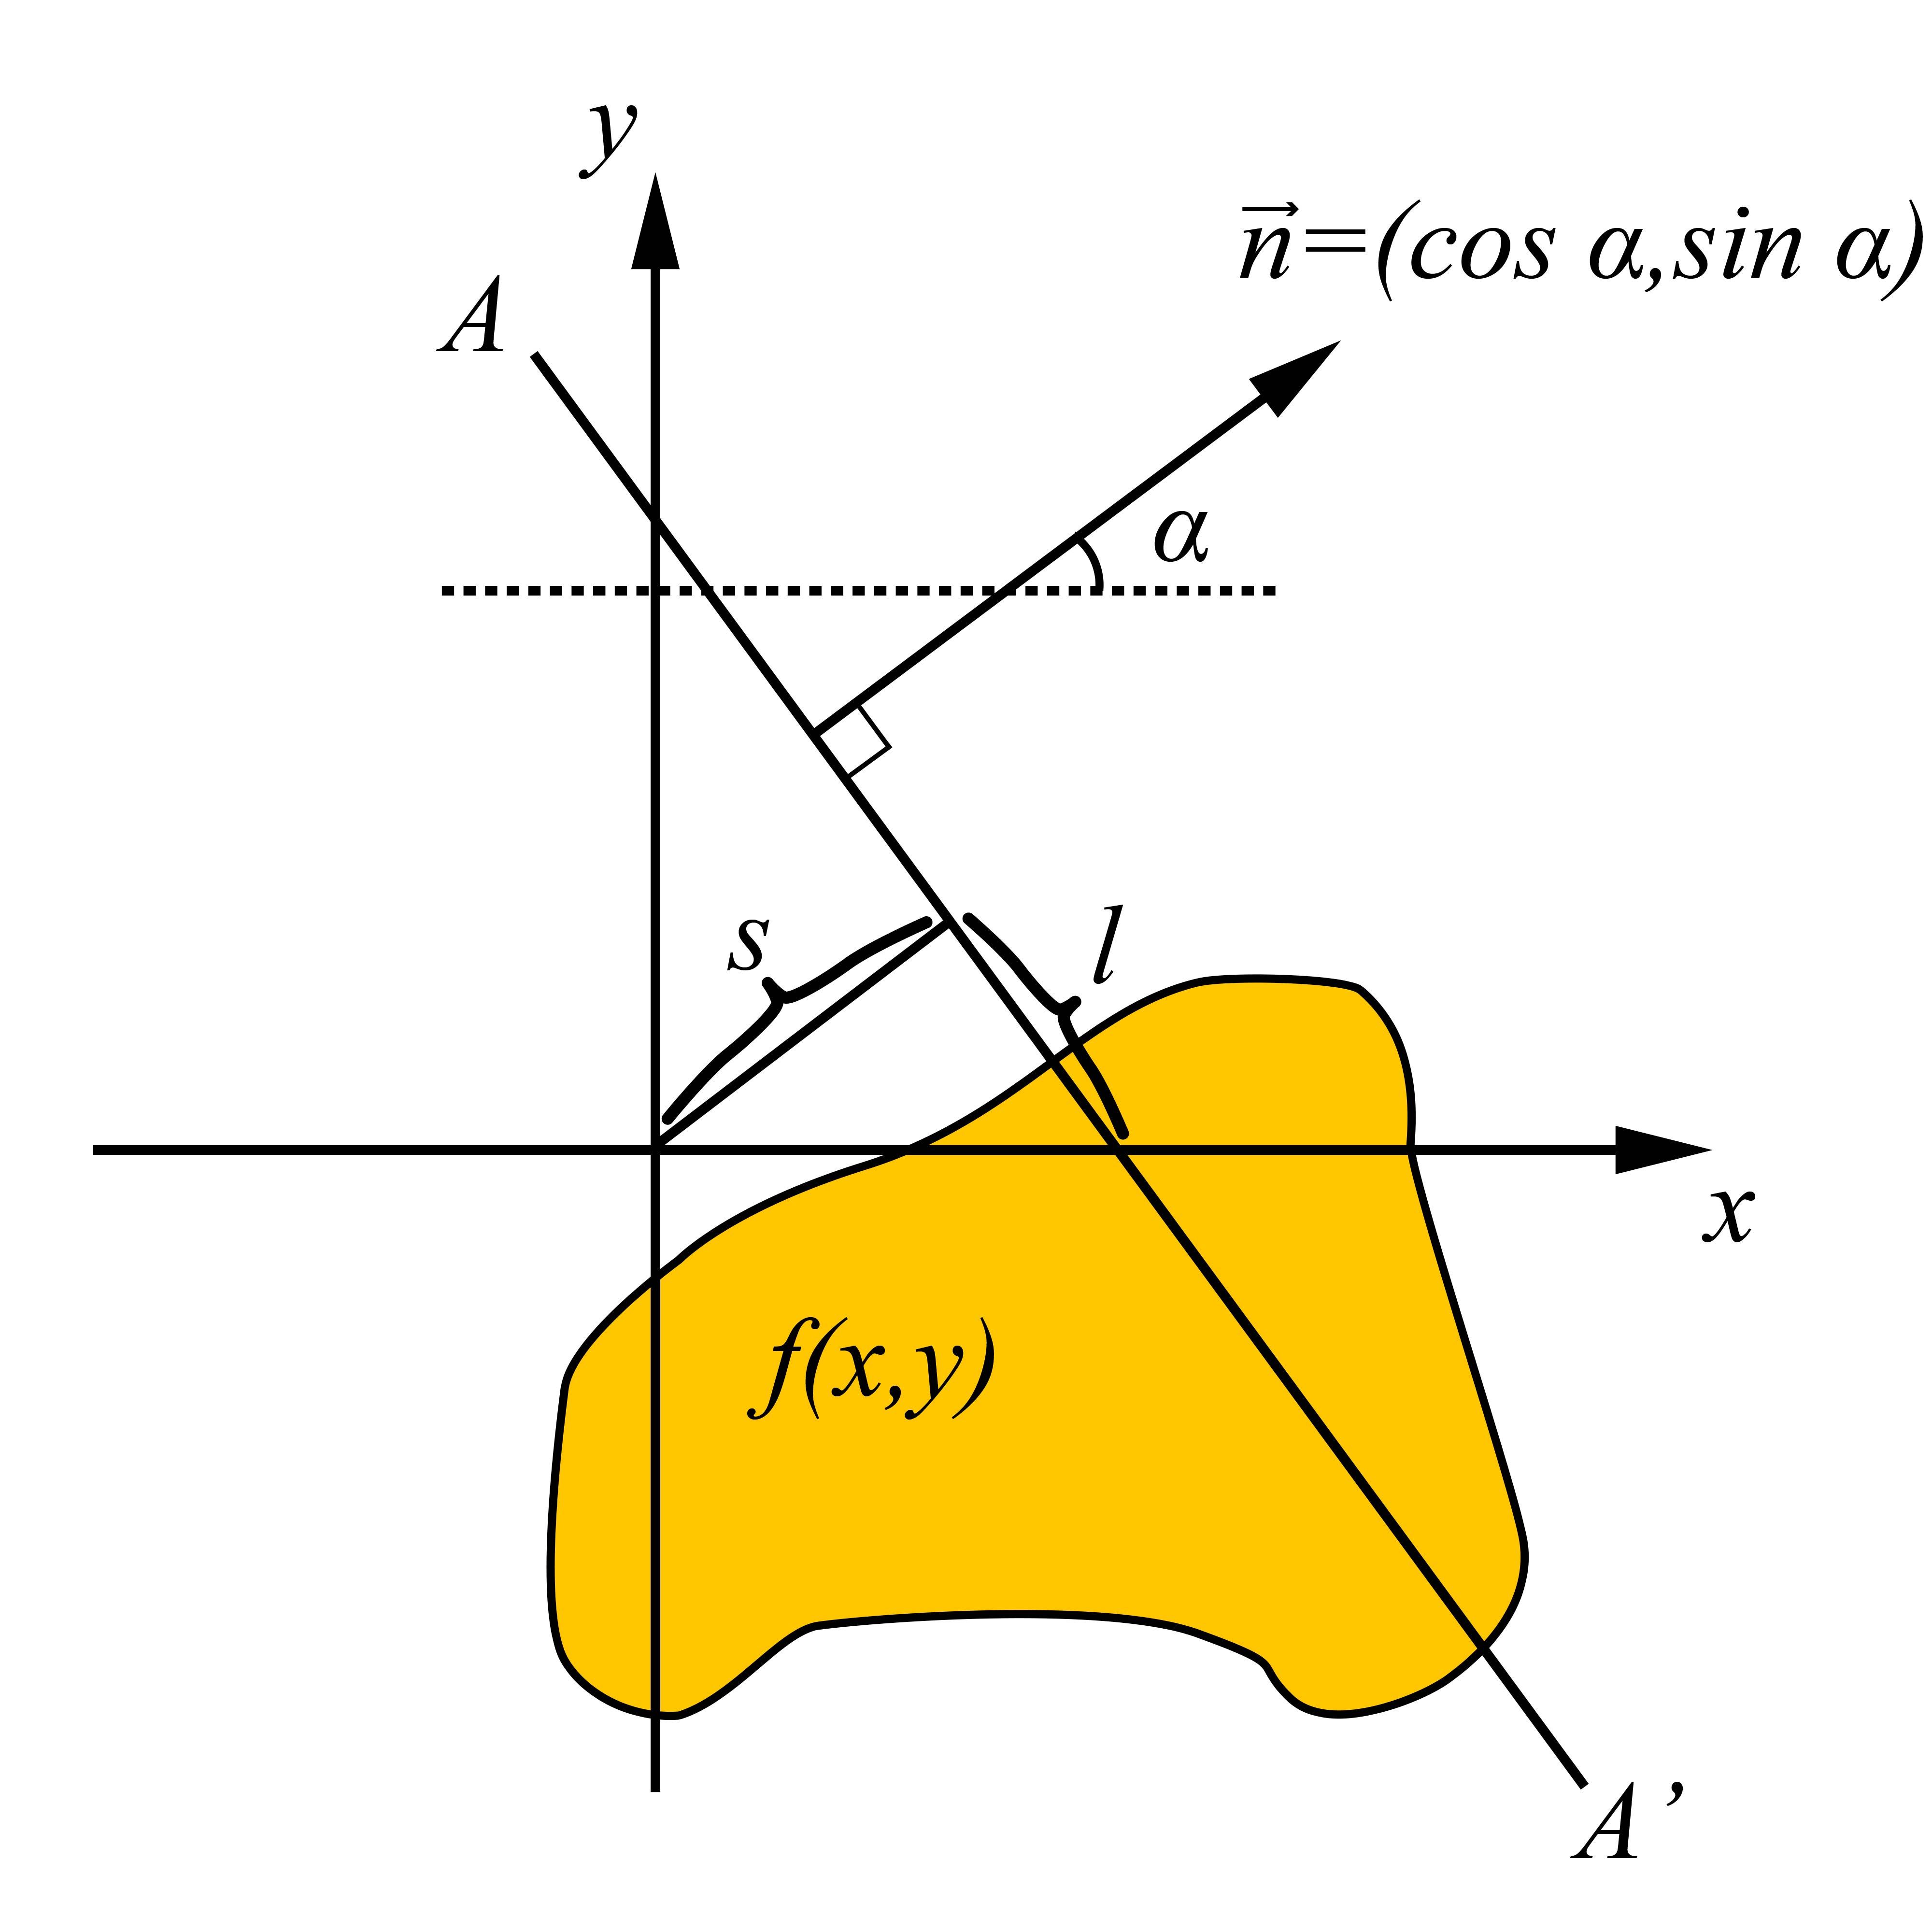
\includegraphics[width=0.4\textwidth]{../1.6/16}
	\caption{拉登变换示意图}\label{fig:16}
	\song\tuzhu{函数 $f$ 从 $(x,y)$ 空间变换至 $(\alpha,s)$ 空间}
\end{figure}

\subsubsection{反投影}
反投影的原理如图 1.7 所示,使物体的投影强度沿投影方向反向等值分布(即反拉登变换),形成反投影体,再将各投影方向的反投影体于正确的几何位置叠加。


三维空间中的反投影可用以下形式表示~\cite{Frank2006}:令 $f(x,y,z)$ 为一个三维物体的空间分布函数,$\boldsymbol{r}=(x,y,z)$ 为空间坐标系。当物体 $f$ 首先围绕 $z$ 轴旋转角度 $\phi_j$,再沿新的 $y$ 轴旋转角度 $\textnormal{-}\theta_j$,最后沿新的 $z$ 轴($z^j$轴)投影至平面 $(x^j,y^j )$ 时,投影
\begin{equation}
p_j=\int f(x^j,y^j,z^j)dz^j
\end{equation}
而新的 $r^j=(x^j,y^j,z^j )$ 坐标系可表示为:
\begin{equation}
\boldsymbol{r}^j=D_{\theta_j}\cdot D_{\phi_j} \cdot \boldsymbol{r}
\end{equation}
其中 $D_{\theta_j}$,$D_{\Phi_j}$ 为旋转矩阵:
\begin{equation}D_{\theta_{j}}=\left(\begin{array}{ccc}
\cos \theta_{j} & 0 & \textnormal{-}\sin \theta_{j} \\
0 & 1 & 0 \\
\sin \theta_{j} & 0 & \cos \theta_{j}
\end{array}\right), D_{\phi_{j}}=\left(\begin{array}{ccc}
\cos \phi_{j} & \sin \phi_{j} & 0 \\
\textnormal{-}\sin \phi_{j} & \cos \phi_{j} & 0 \\
0 & 0 & 1
\end{array}\right)\end{equation}



反投影的投射函数可用下式表示:
\begin{equation}
l_j=\delta(x^j,y^j)c(z^j)
\end{equation}
其中

\begin{equation}c(z^j)=\left\{\begin{array}{cc}
1 & \text { for }-a \leq z^{j} \leq+a \\
0 & \text { otherwise }
\end{array}\right.\end{equation}
参数 $a$ 一般定义为物体的直径。然后将 $p_j$ 反投影,即是将其与 $l_j$ 作卷积:
\begin{equation}
p_j^b(x^j,y^j,z^j)=p_j \otimes l_j
\end{equation}
最后将所有角度下的 $p_j^b$ 相加可以得到重构结果:
\begin{equation}
b(x,y,z)=\sum_j p_j^b (x^j, y^j, z^j)
\end{equation}

值得注意的是,当 $f(x,y,z)$ 为一个狄拉克方程 $\delta$,即中心点为“1”,其余都是“0”时:
\begin{equation}
f(x,y,z) = \delta (x,y,z)
\end{equation}
\begin{equation}
p_j^b(x^j,y^j,z^j)=\delta (x^j,y^j)c(z^j)
\end{equation}
\begin{equation}
b(x,y,z)=\sum_j \delta(x^j,y^j)c(z^j)
\end{equation}
可发现,$b(x,y,z)$ 与 $f(x,y,z)$ 是不相同的。一个点的投影,通过反投影重构后并不是一个点。反投影的重构结果可看作原物体与点扩散函数的卷积。为了求解真实的原物体,需要对反投影中的点扩散函数解卷积。

\begin{figure}[htbp]
	\vspace{\baselineskip}
	\centering
	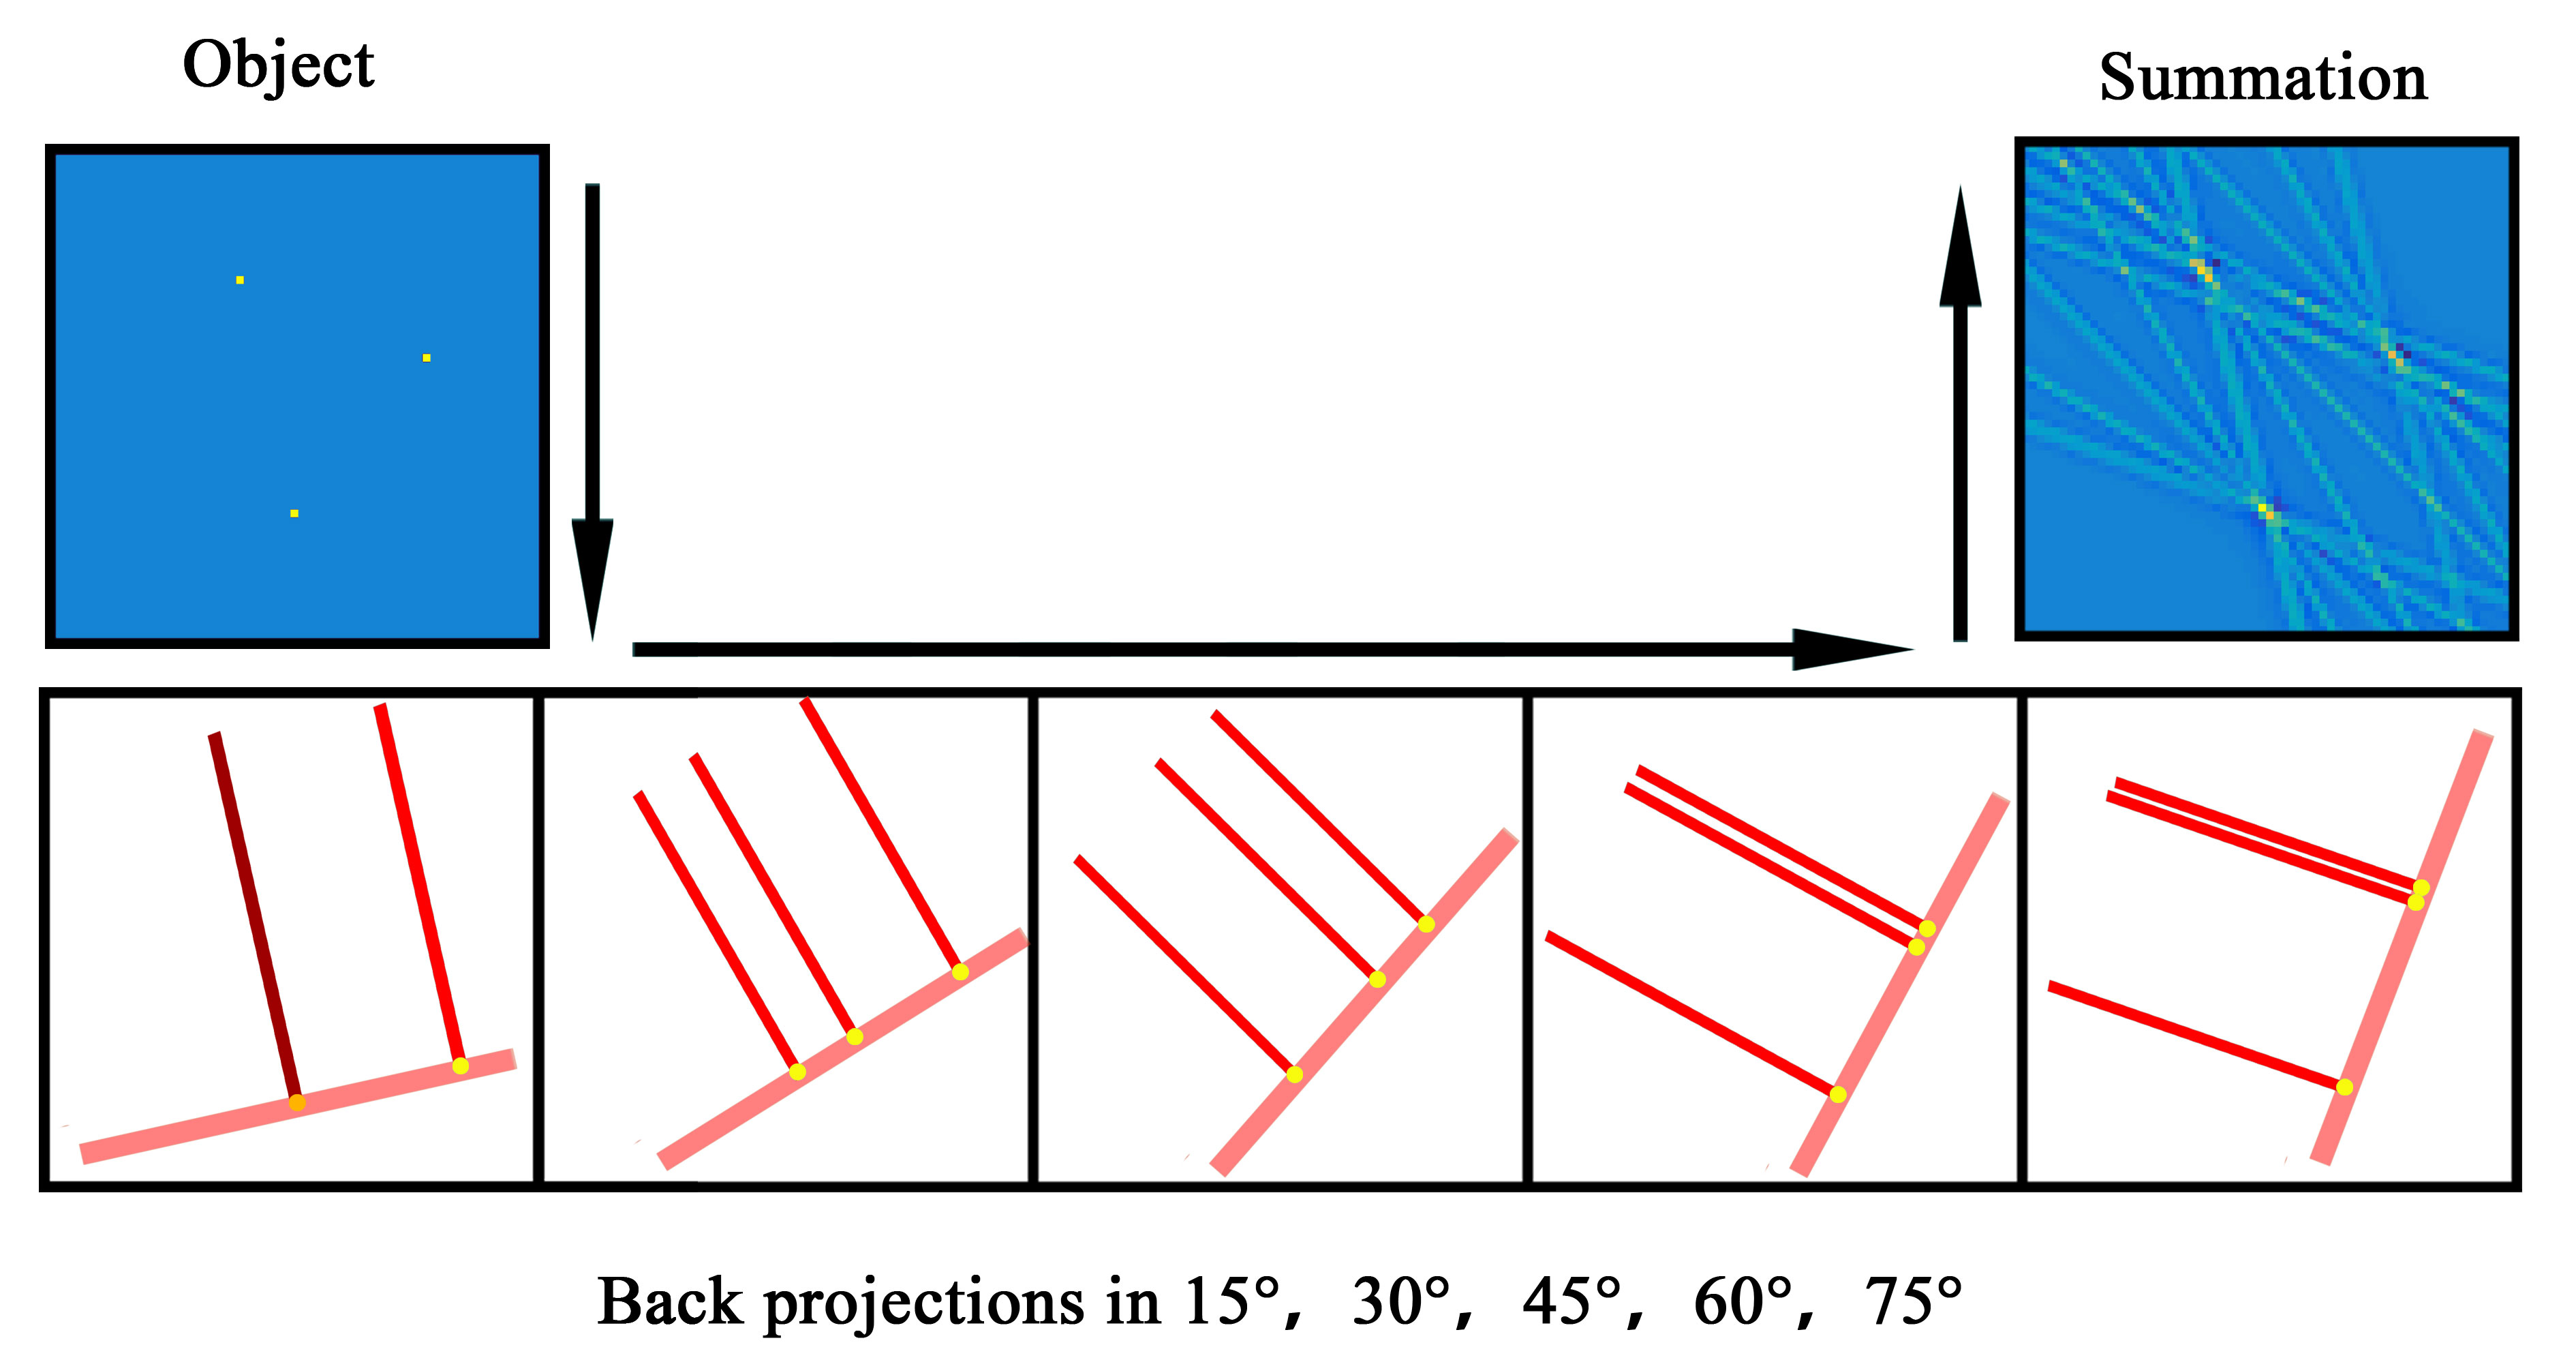
\includegraphics[width=0.8\textwidth]{../1.7/17}
	\caption{反投影原理二维示意图}\label{fig:17}
\end{figure}

\subsubsection{滤波反投影(FBP)}
FBP~\cite{Kak1988}是 3DET 中 最常用的算法,它的做法是先将投影进行滤波,再对其做反投影。常用的滤波器分别为:
\begin{equation}
\text{ramp filter:} f(k)=2\pi k
\end{equation}
\begin{equation}
\text{shepp-logan filter:} f(k)=\sin  k / k
\end{equation}
\begin{equation}
\text{cosine filter:} f(k)=\cos k
\end{equation}
\begin{equation}
\text{hamming filter:} f(k)=0.54+0.46\times \cos k
\end{equation}
\begin{equation}
\text{hann filter:} f(k)= \frac{1}{2} \left(1+\cos k\right)
\end{equation}
滤波的作用即是对公式(1.36)中的点扩散函数解卷积的一种近似操作。
\subsubsection{权重反投影(WBP)}
实际的点扩散函数和实验中具体的倾转模式有关,因此精确的解卷积是复杂的。WBP 的做法是依据具体的倾转模式计算出一个权重滤波器,将此滤波器与反投影的结果卷积以消除点扩散函数的影响。

权重滤波器的构造方法为~\cite{Wolf2014}:首先构造中心像素点为“1”,其余像素点为“0”的图形(如图 1.8a),将其按照实际实验中的倾转角度做倾转投影。然后使用反投影,对这些投影重构得到图 1.8b,重构的结果实际为此倾转模式下的点扩散函数。将这个点扩散函数进行傅里叶变换,得到传递函数(transfer function,TF)。为了避免除零问题和强烈的噪音,该传递函数必须取阈值。最终,权重滤波器为传递函数的倒数。阈值为:
\begin{equation}
t=\textit{TF}(0,0)/N_{\alpha}
\end{equation}
其中 $N_{\alpha}$ 为倾转角个数,$\textit{TF}(0,0)$ 是传递函数原点的数值。
\begin{figure}[htbp]
	\vspace{\baselineskip}
	\centering
	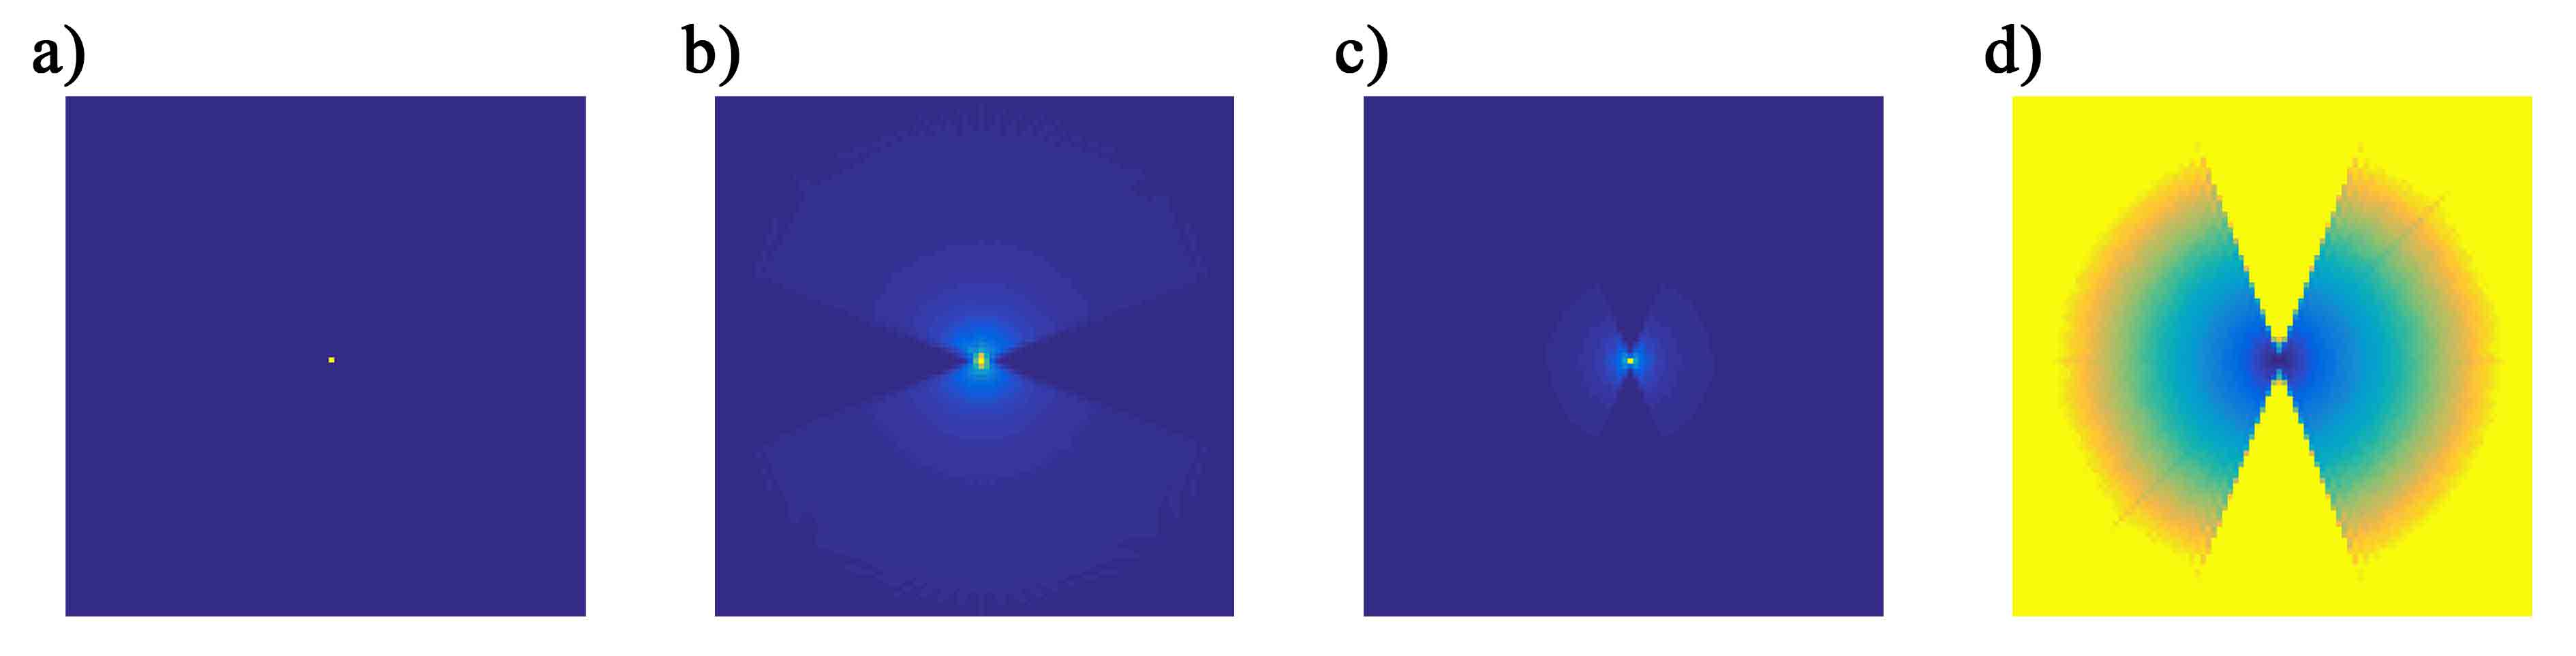
\includegraphics[width=0.8\textwidth]{../1.8/18}
	\caption{权重滤波器构造示意图}\label{fig:18}
	\song\tuzhu{a) 构造中心像素点为“1”,其余像素点为“0”的图形;b) 点扩散函数;c) TF;d) 权重滤波器}
\end{figure}

\subsection{代数法}
\subsubsection{代数重构技术(ART)}
Kaczmarz 算法是波兰数学家 S. Kaczmarz 发明的一种求解线性方程组(公式 1.43)的迭代算法~\cite{Kaczmarz1937}。1970 年,R. Gordon、R. Bender 和 G.T. Herman 将该算法应用于图像重构领域,并称其为 ART~\cite{Gordon1970}。ART 算法包含正约束,是一种非线性的求解方法。ART 算法相比于其他算法的一个优势是易于在重构过程中引入先验知识。

物体沿不同方向的投影是一个线性变换的过程,用以下公式表示这个过程:
\begin{equation}
\boldsymbol{Ax=b}
\end{equation}
其中 $\boldsymbol{b}\left(=(b_1,b_2,\cdots,b_M)^T(\in\mathbb{R}^M)\right)$ 表示观察到的投影数据,即  sinogram; $\boldsymbol{x}\left(=(x_1,x_2,\cdots,x_N)^T(\in\mathbb{R}^N)\right)$  表示被投影的物体的像素;$A\left(=A(i,j)\right)$ 是一个 $M\times N$ 的稀疏矩阵,它表示 $\boldsymbol{x}$ 中的每个像素点在投影过程中对 $\boldsymbol{b}$ 中每个数据的相对贡献。在已知 $\boldsymbol{A}$ 和 $\boldsymbol{b}$ 的情况下,当 $M<N$ 时,求解 $\boldsymbol{x}$ 是求解欠定线性方程组的过程,没有稳定、唯一的解,是一个非适定的反问题。ART 根据下式计算此线性方程组的近似解:
\begin{equation}
\boldsymbol{x}^{k+1}=\boldsymbol{x}^k+\lambda_k \frac{b_i-\langle a_i,\boldsymbol{x}^k \rangle}{\| a_i\|^2}a_i^T
\end{equation}
其中 $i=k \mod M+1$,$a_i$ 是矩阵 $\boldsymbol{A}$ 的第 $i$ 行,$b_i$ 是矢量 $\boldsymbol{b}$ 的第 $i$ 个分量,$\lambda_k$ 是弛豫参数,$0<\lambda_k \leq 1$。弛豫参数的作用是减慢算法的收敛速度,尽管计算时间将增加,但是可以加强重构结果的信噪比。

\subsubsection{同时迭代重构技术(SIRT)}
根据公式(1.44),$\boldsymbol{x}^k$ 的更新误差 $\frac{b_i-\langle a_i,\boldsymbol{x}^k \rangle}{\| a_i\|^2}a_i^T$ 是 $\boldsymbol{x}^k$ 到超平面 \(a_i\boldsymbol{x}^{\prime}=b_i\) 的投影距离。在 ART 中,每计算一次误差,$\boldsymbol{x}$ 都会更新。在 SIRT 中,$\boldsymbol{x}$ 只会在计算出所有来自 $M$ 个超平面的总误差之后才会被更新,即~\cite{Andersen1984,Kak1988}:
\begin{equation}
\boldsymbol{x}^{k+1}_i = \boldsymbol{x}^k_i + \frac{\sum_j\left[a_{ij}\frac{\sum_ix_i^ka_{ij}-a_j^T\boldsymbol{x}^k}{\sum_ia_{ij}}\right]}{\sum_ja_{ij}}
\end{equation}

\subsection{傅里叶变换法}
\subsubsection{傅里叶中心切片定理}
傅里叶中心切片定理的定义是,物体三维傅里叶变换的中心截面等同于物体投影的二维傅里叶变换。可以通过以下公式证明~\cite{Frank2006}:
\begin{equation}
F(X,Y,Z)=\iiint_{object} f(x,y,z)\exp \left(2\pi i(xX+yY+zZ)\right)dxdydz
\end{equation}
其中 $f(x,y,z)$ 代表实空间中的物体,$F(X,Y,Z)$ 表示物体的三维傅里叶变换。而 $F(X,Y,Z)$ 在中心截面 $Z=0$ 处为:
\begin{equation}
F(X,Y,0) = \iint \sigma(x,y)\exp\left(2\pi i (xX+yY)\right)dxdy
\end{equation}
\begin{equation}
\sigma(x,y)=\int f(x,y,z)dz
\end{equation}
$\sigma(x,y)$ 为物体沿 $z$ 轴的投影,得证。

傅里叶中心切片定理在应用上存在一个问题,实验所获得的倾转系列像的数据排列在以倾转轴为原点的极坐标中,而计算机数值计算过程中的三维体矩阵是均布于笛卡尔坐标系,两个坐标系之间的数值转换需要插值,易造成较大误差。为此,基于极坐标与伪极坐标的傅里叶变换方法被引入到三维重构的算法之中,相比于笛卡尔坐标系中的快速傅里叶变换算法,这些算法牺牲了运算速率,但是克服了两个坐标系之间数值转换的问题,提高了计算精度。

\subsubsection{等斜率技术(EST)}
EST 基于傅里叶中心切片定理,该方法通过伪极傅里叶变换~\cite{Averbuch2006}实现了以极坐标分布的实验数据与到笛卡尔坐标系中的重构结果之间的数学空间变换。由于伪极坐标(如图 1.9 所示)中的极角以等斜率的方式排布,因此得名。
该方法首先使用零填充和分数傅里叶变换,将每个极角所在的实验数据变换到伪极坐标的格点上,得到过采样的傅里叶片层(Fourier slice)。分数傅里叶变换的定义如下:
\begin{equation}
F_{\alpha}(\boldsymbol{k})=\sum_{x=-N}^{N-1}f(\boldsymbol{r})\exp\left(-\frac{i\pi\alpha\boldsymbol{k}\boldsymbol{r}}{N}\right)
\end{equation}
其中 $\boldsymbol{k}$ 为傅里叶空间坐标,$\boldsymbol{r}$ 为实空间坐标,$N$ 为实验数据的采样数。$f(\boldsymbol{r})$ 代表实验数据,$F_{\alpha} (\boldsymbol{k})$ 代表傅里叶片层。$\alpha$ 是一个适配因子,$\alpha$ 选取合适的数值,以在不同极角下将实验数据样变换到伪极格点上。

\begin{figure}[htbp]
	\vspace{\baselineskip}
	\centering
	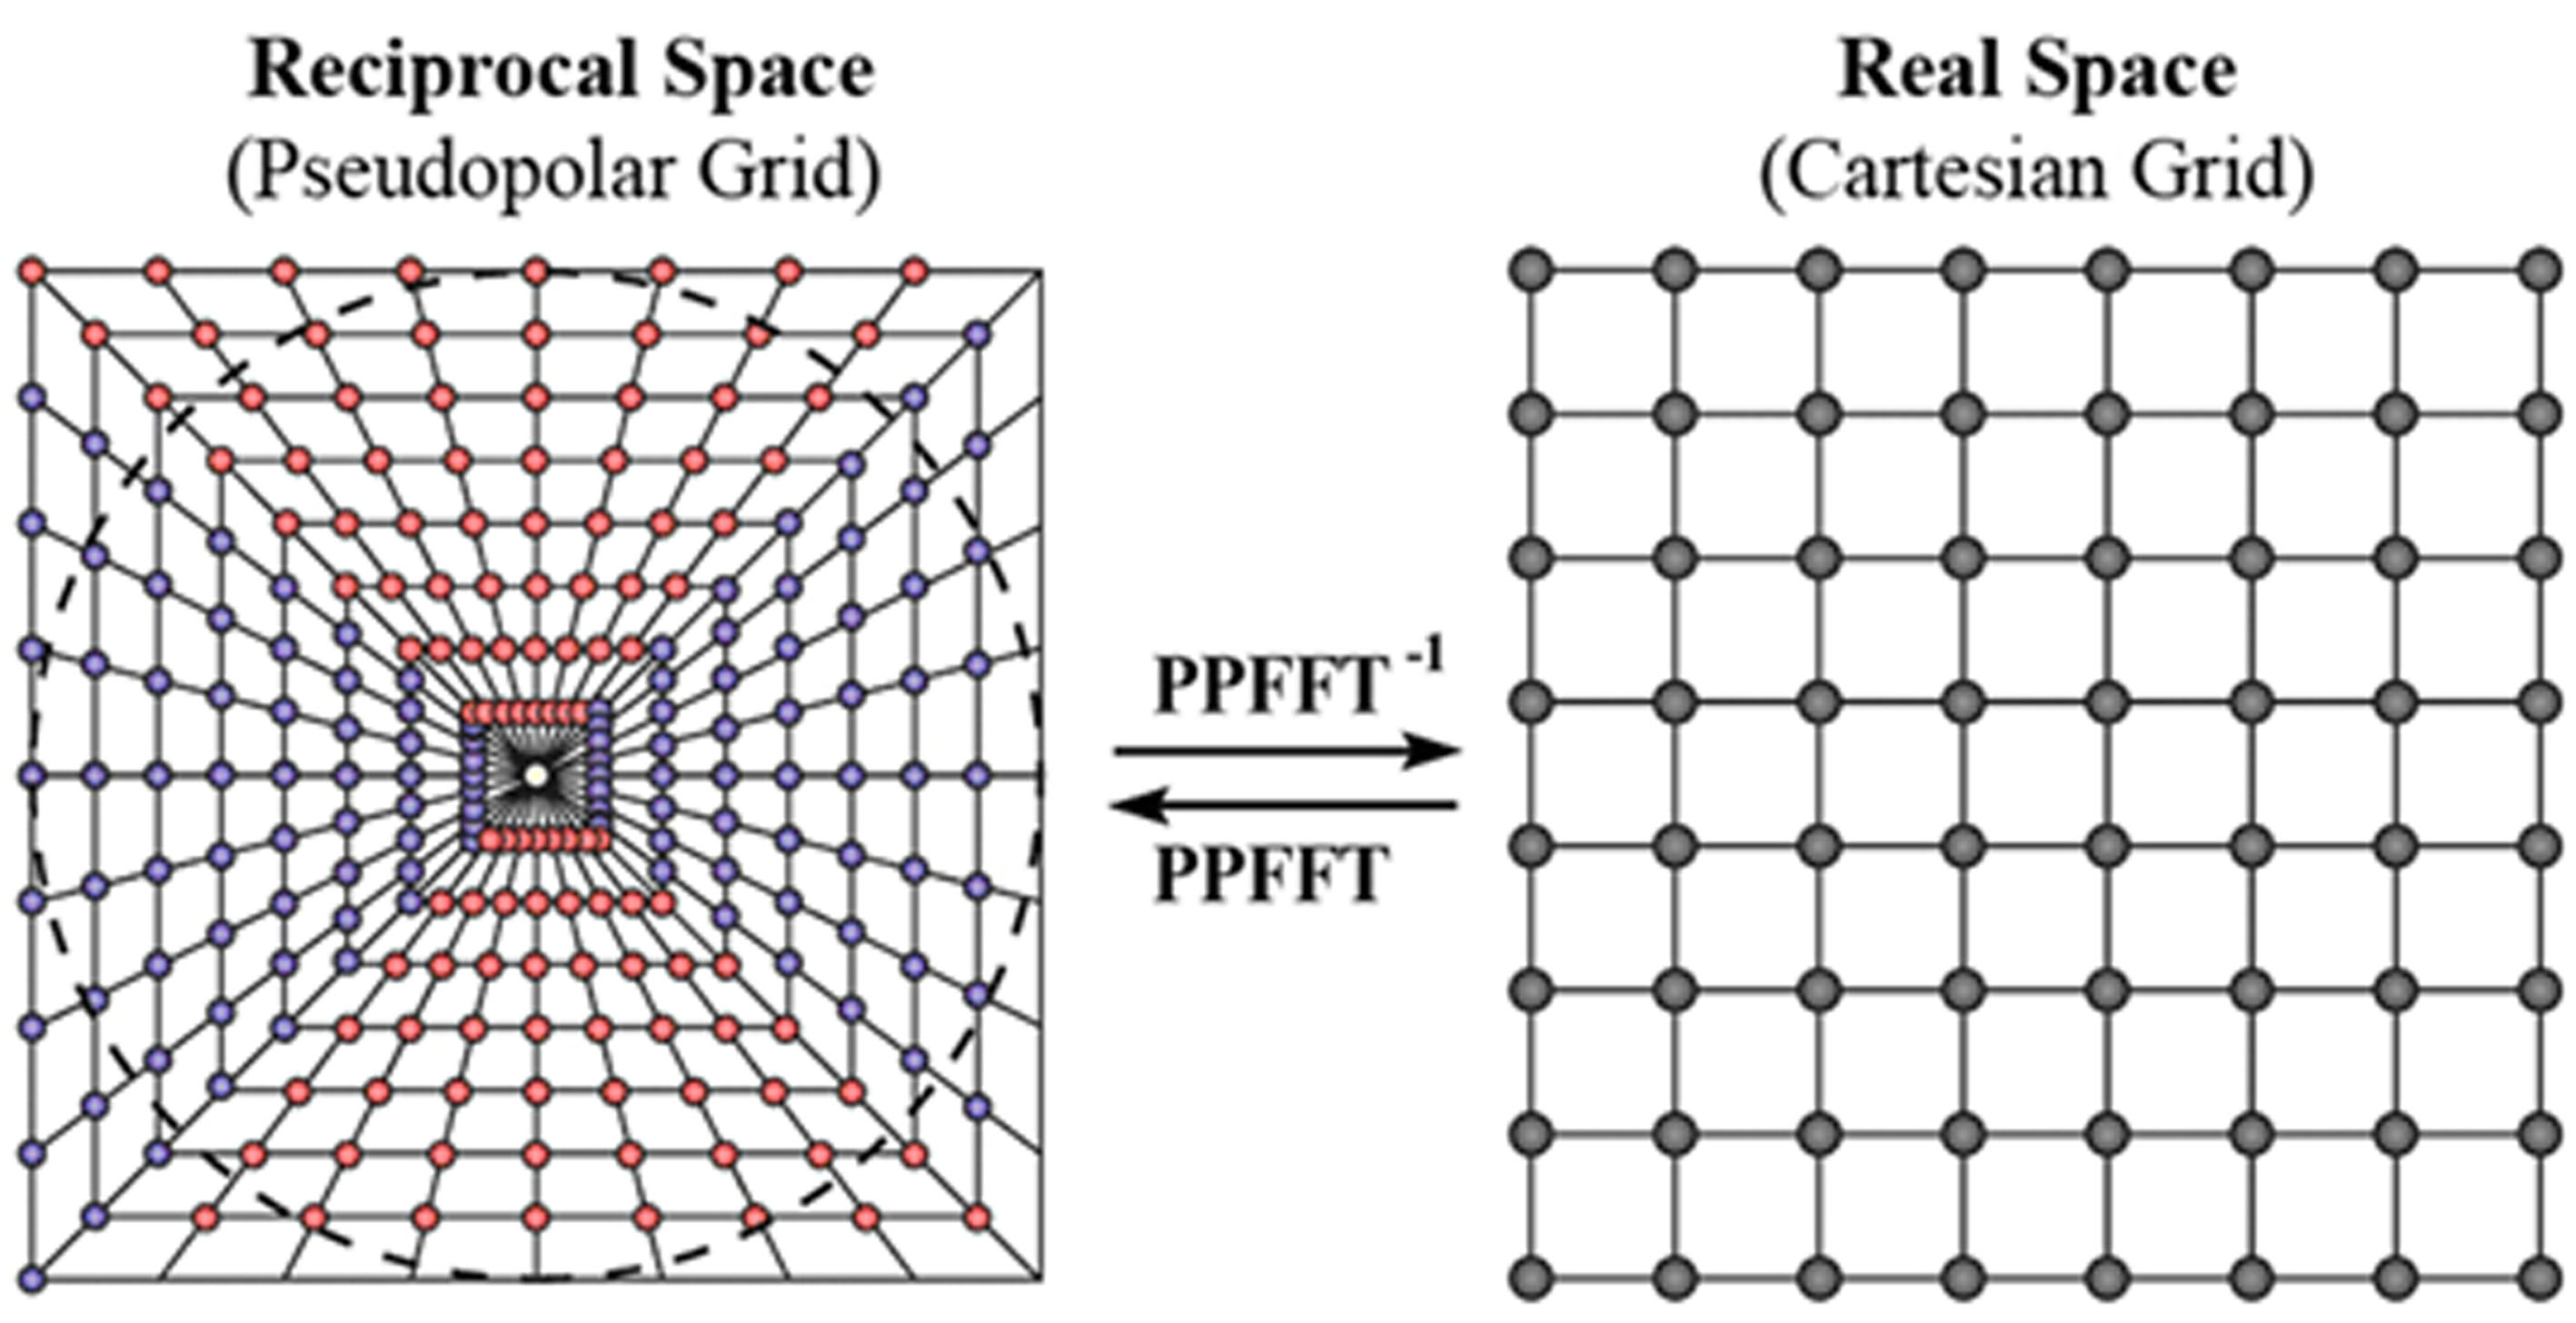
\includegraphics[width=0.8\textwidth]{../1.9/1_9}
	\caption{伪极傅里叶坐标系与笛卡尔坐标系的转换图$^{[21]}$}\label{fig:19}
\end{figure}

EST 的具体流程为:1.将计算得到的傅里叶片层赋值到构造好的伪极格点上,实验数据不包含的极角的信息都填充为零。
2.将所有在傅里叶空间中的信息,通过伪极傅里叶逆变换,变换到笛卡尔坐标系的实空间中,得到重构结果。3.将这个结果中数值为负的数据全部设为零,再使用伪极傅里叶变换,将其变换回伪极傅里叶空间中。此时,原来实验数据不包含的极角处的数据不再为零,即重构出了未采样处的信息。将实验数据对应的傅里叶片层,替换掉此时的数据。重复2-3步骤,通过迭代的伪极傅里叶变换和数据替换,优化重构结果。

\subsection{正则化方法}
正则化是一种通过引入先验知识来求解不适定问题的方法。在 3DET 的迭代算法中,通常会将正则化项引入误差函数(也称为能量函数)中。比如在 Green 通过最大似然法推导出的 ART 算法中~\cite{Green1990}:
\begin{equation}
x_i^{k+1} = \frac{x_i^k}{\sum_ja_{ij}+\beta(\partial/\partial x_i)U(x^n)}\sum_j \frac{a_{ij}b_j}{\sum_k a_k x_k^n}
\end{equation}
 $U$ 是能量函数,迭代的目的是使系统的能量达到最小。$\beta$ 代表了先验知识与预测函数之间的相对大小。当 $\beta$ 趋近于零时,公式(1.50)就成为了标准的最大似然法。能量函数 $U$ 决定了目标函数的性质,能量函数 $U$ 的形式决定了最终图像的平滑程度~\cite{Persson2001}。

能量函数的形式有很多种,最常见的有 $L_1$ 和 $L_2$ 范数。在 3DET 中,最有效的是全变分(total variation,TV)范数,如下式:
\begin{equation}
\textit{TV}(f) = \int_{\Omega}  |\nabla f|dxdy= \int_{\Omega}\sqrt{f_x^2+f_y^2}dxdy
\end{equation}
TV 项具有非常好的降噪和抑制缺失锥假象的功能。
\begin{figure}[htbp]
	\vspace{\baselineskip}
	\centering
	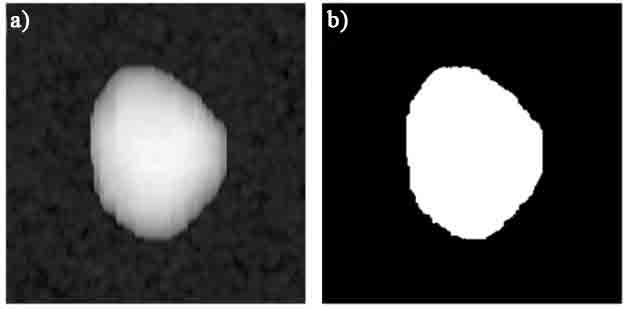
\includegraphics[width=0.8\textwidth]{../1.20/1201}
	\caption{离散代数重构技术示意图$^{[112]}$}\label{fig:120}
	\song\tuzhu{a) 普通重构的结果;b) 离散代数重构技术重构的结果}
\end{figure}

正则化项的引入实际是在重构的迭代过程中,给重构结果加上约束条件。为了达到约束的目的,有些方法比正则化方法更加直接。比如离散代数重构技术(discrete algebraic reconstruction technique,DART)~\cite{Batenburg2009,Bals2007,Biermans2010,Bals2009,Zurner2009,Zhuge2017}直接在重构的过程中对重构结果进行二值化,如图 1.10 所示。该方法在重构一些固定成分的材料时显得尤为有效。


\subsection{基于神经网络的重构方法}
神经网络是 20 世纪 80 年代以来人工智能领域兴起的研究热点。神经网络是一种运算模型,由大量节点之间的互相连接构成,是对人脑神经元网络的抽象。早在 20 世纪 90 年代,就有学者探究神经网络在 CT 图像重建中的应用。当时还没有深度学习的概念,神经网络被当作一个复杂高效的数学优化方法,用于求解公式(1.43),即这是一种 ART 型的神经网络图像重建算法~\cite{Srinivasan1993,Ma2000,Deming1998,Cichocki1995,Wang2006,Teranishi2016}。局限于当时的计算机硬件条件,这方面的研究并没有取得重大的突破。

近年来,得益于计算机设备的飞速发展,神经网络可以达到庞大复杂的网络构型,它以深度学习技术的形式重新回到人们的视野,并在生物、医学、经济等诸多领域解决了现代计算机难以解决的实际问题。已有一些学者开始研究如何利用深度学习技术实现 3DET,并取得了一些不错的进展~\cite{Ding2019,Pelt2013,Bladt2015,YangF2015}。

\subsubsection{ART 型神经网络图像重建方法}
这一类方法利用神经网络求解公式(1.43),其基本思路是利用神经网络优化预测值,使 $\lVert Ax^{guess}-b^{experiment} \lVert$ 达到最小。如在 M. Teranishi 的论文的 Nerual network collocation method~\cite{Teranishi2016}中,具体表现为使 $\lVert \vec{f}^{MLP}-\vec{g}^{meas} \lVert$ 达到最小。其中 $\vec{f}^{MLP}$ 是神经网络的输出,$\vec{g}^{meas}$ 是实验测量的投影。图 1.11 是该神经网络的构型,它将 $(x,y)$ 坐标作为输入层,将预测的物体在该坐标处的强度值作为输出层,即该网络构成了一个物体与空间坐标之间的函数关系。这个关系的具体表达式为:
\begin{equation}
o^h_k = \sigma(w^h_{k,x}x_j + w^h_{k,y}y_j + w^h_{k,b})
\end{equation}
其中 $k$ 表示隐藏层中的某一个节点,$j$ 表示空间中某一个坐标点,$w^h_{k,x}x_j$,$w^h_{k,y}y_j$,$w^h_{k,b}$ 分别表示隐藏层中的权重和偏置,$\sigma$ 是 sigmoid 函数 $\sigma(u)=1/(1+e^{-u})$。于是:
\begin{equation}
f^{MLP}(\vec{w}, x_j,y_j)= \sigma \sum_{k}(w^o_{k,x}o^h_k + w^o_{k,b})
\end{equation}
$w^o_{k,x}$ 和 $w^o_{k,b}$ 是输出层的权重和偏置,$\vec{w}$ 则是所有权重和偏置的集合矢量。然后定义误差函数:
\begin{equation}
E^{prj} = \frac{1}{2}\sum_{i}(g_i^{MLP}-g_i^{meas})^2
\end{equation}
其中 $g_i^{MLP}$ 是根据 $f^{MLP}(x_j,y_j)$ 沿第 $i$ 个投影方向计算的投影数据。为了使 $E^{prj}$ 达到最小,使用梯度下降算法优化 $\vec{w}$,即:
\begin{equation}
\vec{w}^{(t+1)} = \vec{w}^{(t)} + \Delta \vec{w}^{(t)}
\end{equation}

\begin{equation}
\Delta \vec{w}^{(t)} = -\eta \frac{\partial E^{prj}}{\partial \vec{w}^{(t)}} + \beta \vec{w}^{(t-1)}
\end{equation}
其中 $\eta$ 是学习率,$\beta$ 是历史学习动量因子。

\begin{figure}[htbp]
	\vspace{\baselineskip}
	\centering
	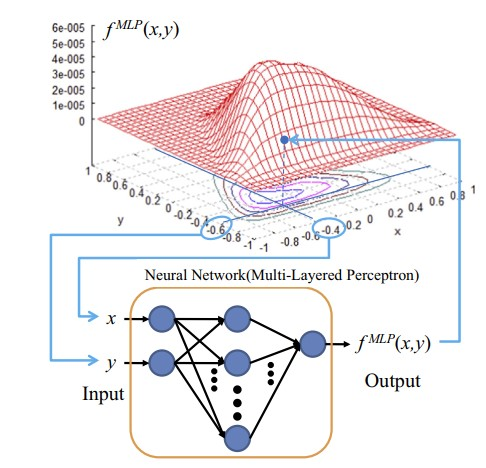
\includegraphics[width=0.5\textwidth]{../1.17/117}
	\caption{Nerual network collocation method 示意图$^{[118]}$}\label{fig:117}
\end{figure}

ART 型的神经网络重构算法的基本思路相同,具体网络构型可以有较多变化,本节中仅以上述方法为例作简单介绍。

\subsubsection{深度学习的 3DET 方法}
深度学习方法的主要思路是用大量实例训练神经网络模型,使这个模型面对新的实验数据时能快速计算出正确的重构结果。以 E. Bladt 等论文~\cite{Bladt2015}中的 neural network filtered backprojection 方法为例。如图 1.12 所示,在 learning phase 中,需要使用大量已知结构的高质量投影图像作为神经网络的输入层,对网络进行训练。训练得到的一系列模型作为新数据重构需要的滤波器。在 reconstruction phase 中使用这些滤波器对新的实验数据进行滤波等操作,最终可以快速得到重构结果。并且,这些滤波器只需要少量的实验投影图像就能得到良好的重构结果。

而在 G.L. Ding 等的论文~\cite{Ding2019}中,如图 1.13,他们使用深度学习技术直接补全投影数据缺失的部分来抑制缺失锥效应。补全后的 sinogram 可以使用任意 3DET 算法(比如 FBP、WBP 等最简单的方法)进行重构。

深度学习的 3DET 方法与 ART 型的方法最大的不同是,它花费大量的时间用于“学习”过程,但训练成功的模型可以反复使用。不过,模型可使用的范围与训练集的性质有关,有很大的局限性。

\begin{figure}[H]
	\vspace{\baselineskip}
	\centering
	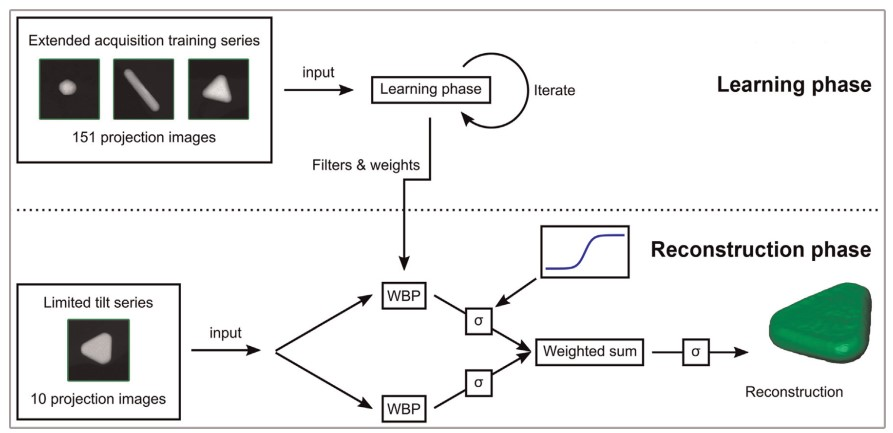
\includegraphics[width=0.8\textwidth]{../1.18/118}
	\caption{Neural network filtered backprojection 方法示意图$^{[121]}$}\label{fig:118}
\end{figure}

\begin{figure}[H]
	\vspace{\baselineskip}
	\centering
	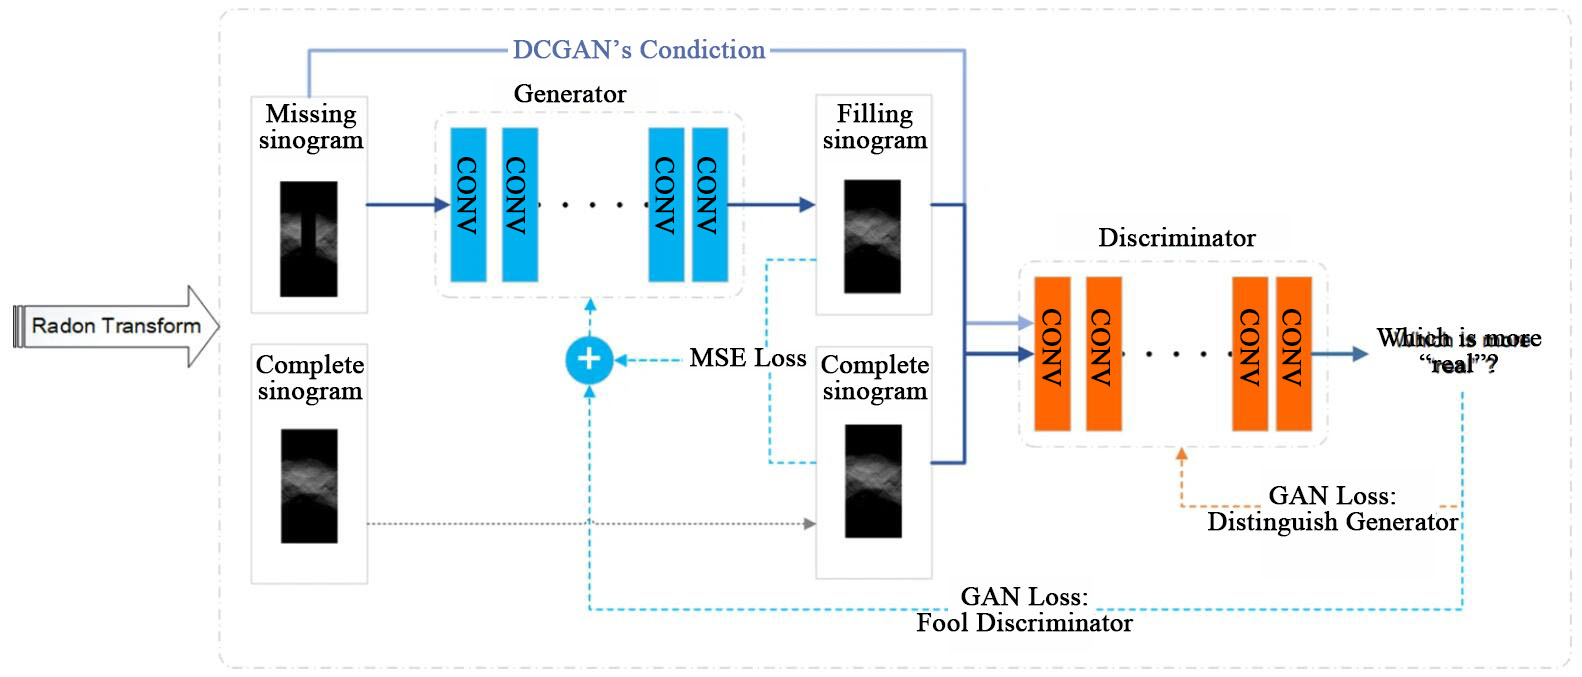
\includegraphics[width=0.8\textwidth]{../1.19/119}
	\caption{深度学习补全 sinogram 的算法流程图$^{[119]}$}\label{fig:119}
\end{figure}

\subsection{样品漂移配准}
通常,一套 3DET 实验倾转系列像包含 100 多张 STEM 图像,收集时间需要几个小时。在对样品进行倾转和拍摄时,样品在电镜中的漂移是不可避免的。样品漂移的原因有很多,比如设备的机械振动,样品由于电子束轰击发热等。在三维重构之前,需要对倾转系列像进行配准,消除图像之间的漂移。

配准的方法可以分为两大类,基准标记~\cite{Ress1999,Brandt2001}和相关法~\cite{Ress1999,Jones2013}。基准标记法在样品制备过程中加入基准标记,通常为金颗粒。在实验过程中,这些标记与样品的相对位置是不变的,所以标记的位置变化就对应于样品的漂移。在图像的配准过程中,只需要追踪一定数量的标记位置,就可以矫正图像的漂移。基准标记法的主要优点是它确定的漂移量是绝对的漂移量,对于整个倾转系列像是统一的(与相关法形成了鲜明的对比)。遗憾的是,不是所有的样品都适用于这种方法,并且由于金颗粒是重元素材料,有时候它会在重构结果中引入假象。

相关法是另一种行之有效的配准方法。它利用互相关函数计算两张图像之间的偏移量。两张图像的互相关函数是一个二维的矩阵,矩阵中的元素的强度表示这两张图像在该位置的相似度。所以,矩阵中最大值的坐标代表了图像之间的漂移量。根据相关法的原理,相关法计算的两张图像之间需要有很高的相似度,一般使用相关法依次配准相邻倾转角的两张实验像。在 3DET 中,某些片状样品在倾转的过程中,垂直于倾转轴的宽度会发生变化,在进行配准之前,需要矫正这种变化。与基准标记法相比,互相关法计算的是两张图像之间的相对漂移量,整体的漂移校正统一性较差,有时候累计的误差会较大。所以互相关法的配准结果一般需要迭代优化。
\subsection{缺失锥问题}
缺失锥问题是 3DET 中普遍存在的问题。3DET 实验中收集的倾转系列像的倾转角通常不能覆盖全 180°,这会导致三维重构的结果在傅里叶空间中存在一个锥形的信息缺失区域,所以这个问题被称为缺失锥问题。造成缺失锥问题的原因主要有二:1.由于电镜构造的原因,很多透射电镜中的样品台无法全角度旋转,普遍情况是倾转角被限制在 -70° 至 +70° 之间;2.大部分透射电镜样品在倾转到高角度时,由于样品有效厚度增加,已经无法正常地获得电镜照片。

\begin{figure}[htbp]
	\vspace{\baselineskip}
	\centering
	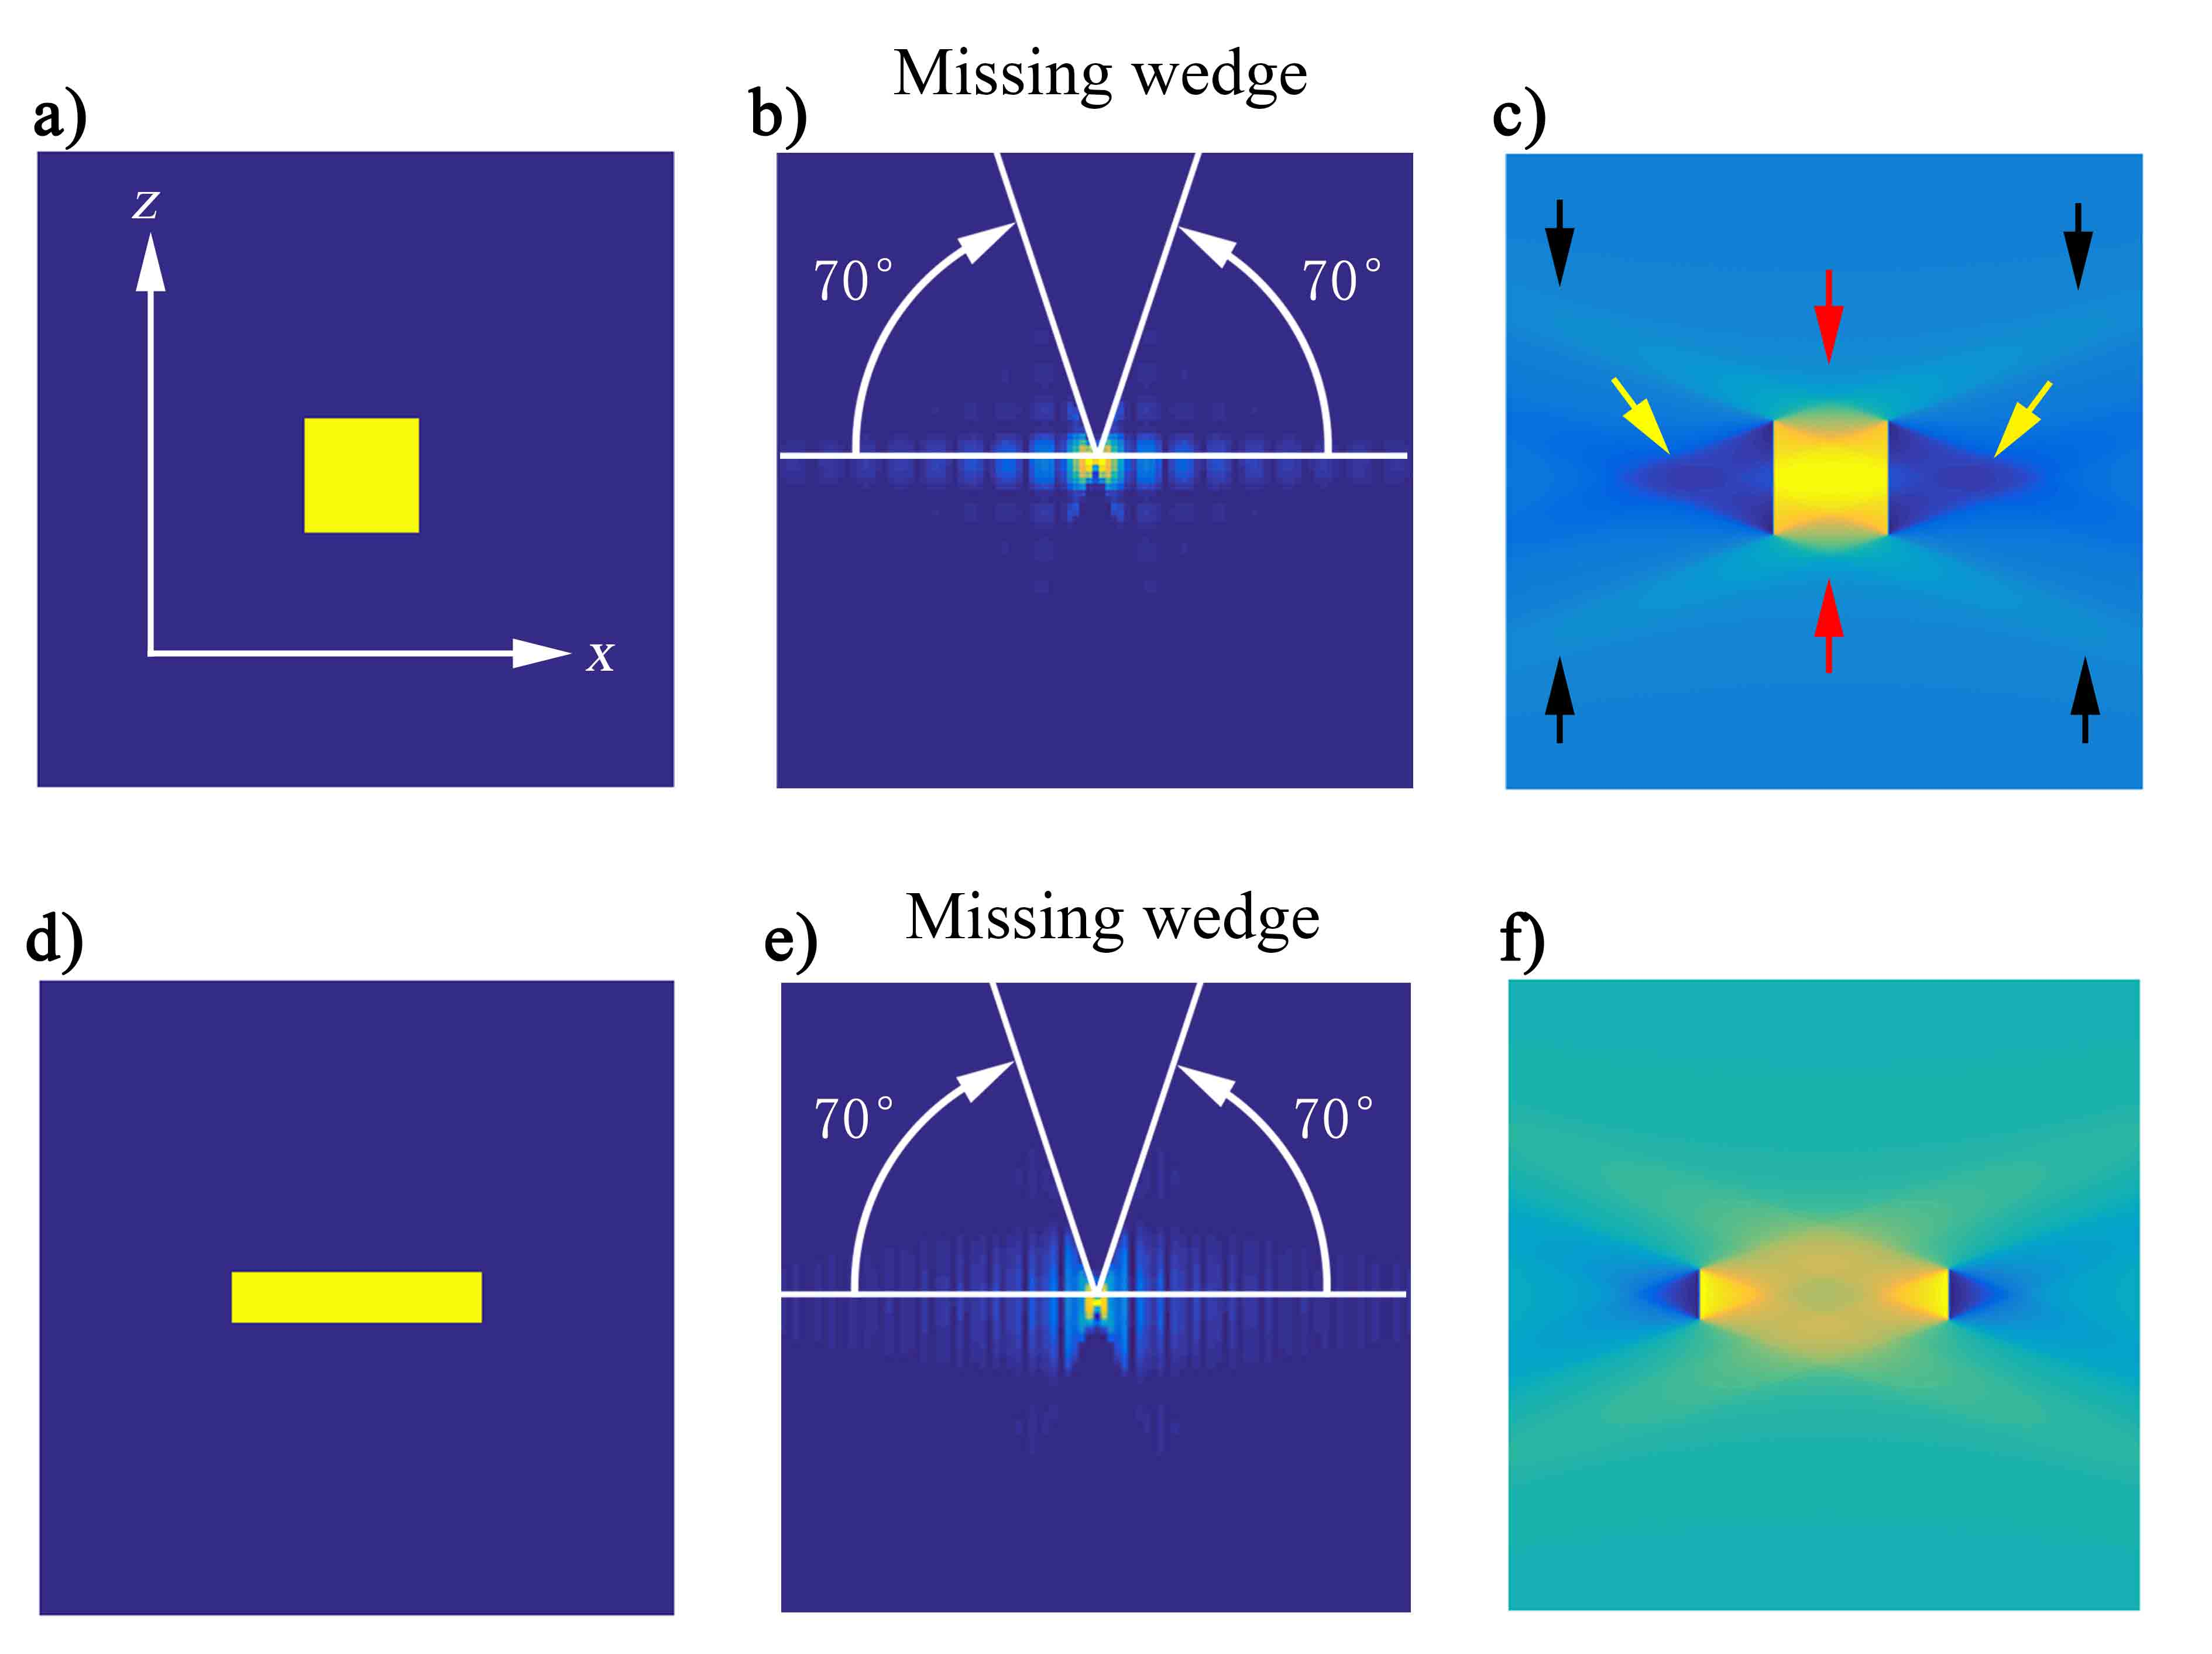
\includegraphics[width=0.8\textwidth]{../1.10/110}
	\caption{缺失锥及其效应的示意图}\label{fig:110}
	\song\tuzhu{a-c) 分别是模拟的正方形和对其投影再重构后的傅里叶空间频谱图和重构图,c 中黑色箭头标注的是射线假象,红色箭头标注的是拉伸假象,黄色箭头标注的是局部低强度假象;d-f) 分别是模拟的纵横比为 5 的长方形和对其投影再重构后的傅里叶空间频谱图和重构图;两次模拟均对模型进行了 -70° 至 +70° 的投影及再重构,傅里叶空间频谱图只展示了中间部分区域,以利于观察}
\end{figure}

缺失锥会在重构的图像中引起三种假象~\cite{Kovacik2014},如图 1.14c 所示:(1)垂直于最大投影倾转角的射线假象,这个假象虽然强度较低,但是在空间中是无限延伸的;(2)重构的物体在 $z$ 方向被拉长;(3)沿 $x$ 轴,在物体两侧出现局部的低强度区域~\cite{Gontard2015}。这些假象会严重影响重构物体的形貌和内部强度,妨碍对三维物体尺寸和形貌的精确测量。此外,缺失锥假象的严重程度,还与物体的外形与倾转角度之间的空间位置有关,对于纵横比大的物体,且其未倾转时长轴垂直于 $z$ 轴时,缺失锥引起的假象将非常严重。如图 1.14d-f 所示,纵横比为 5 的长方形垂直于 $z$ 轴摆放,在 -70° 至 +70° 的投影角度下得到的 sinogram 再经 FBP 重构后,重构结果中长方形形状断开,无法辨识。

在缺失锥存在时,重构的分辨率将被进一步降低,$z$ 方向的分辨率~\cite{Frank2006}:
\begin{equation}
d_z =d\cdot \epsilon
\end{equation}
\begin{equation}
\epsilon=\sqrt{\frac{a_{max}+\cos a_{max}\sin a_{max}}{a_{max}-\cos a_{max} \sin a_{max}}}
\end{equation}
其中 $d$ 为克劳瑟限制中的重构分辨率(见第 1.3.10 条),$a_{max}$ 为最大倾转角度。

\subsection{电镜会聚束的分辨率限制}
HAADF-STEM 是收集样品投影信息最常用的手段。然而,在 STEM 中,电子会聚束的会聚角对 STEM 图像的分辨率具有决定性的影响。为了避免像差对成像的影响,在透射电镜中使用聚光镜光阑遮挡受像差影响过大的电子,而这限制了会聚束的会聚角。

在 STEM 中,电子束束斑的横向分辨率 $d$ 与会聚角 $\alpha$ 的关系为~\cite{Ishikawa2015}:
\begin{equation}
d=0.61\frac{\lambda}{\alpha}
\end{equation}
其中 $\lambda$ 是电子波波长,$\alpha$ 是会聚束的会聚半角。与此同时,垂直于图像平面上的分辨率,也称作景深~\cite{Nellist2007}:
\begin{equation}
d_z=1.77\frac{\lambda}{\alpha^2}
\end{equation}

随着电镜设备与技术的发展,会聚束可达到的会聚角日益增大,这在提高 STEM 成像分辨率的同时带来一个问题,景深越来越小,以至于可重构的样品尺寸越来越小。

\subsection{克劳瑟限制}
在 3DET 实验中收集的投影的数量总是有限的。根据克劳瑟(Crowther)的理论~\cite{Crowther1970},在单轴倾转的模式下,以 $\Delta \theta$ 为等倾转角收集满 180° 的投影时,重构的分辨率为:
\begin{equation}
d=\frac{\pi D}{N}
\end{equation}
其中 $D$ 是物体的直径,$N$ 是投影个数。
由此可知,样品的大小和获取的投影数量会影响重构的分辨率。当重构较大的样品时,需要收集更多的投影以保证足够分辨率。
为了突破克劳瑟限制,R. Hovden 等~\cite{Hovden2014}和 C. Jacobsen 等~\cite{Jacobsen2018}提出将深度剖面方法与断层成像方法结合,增加每个投影方向收集的信息,从而提高重构分辨率。

\section{原子分辨率三维重构新方法}
\subsection{“大爆炸”三维重构}
2012 年,D. Van Dyck 等~\cite{VanDyck2012}提出了一种新的原子分辨率的三维重构方法,“Big Bang”三维重构。如图 1.15 所示,该方法将电子波经原子势场作用后离开原子的传播过程,与宇宙大爆炸后行星系的运动过程相比拟,故得名。根据哈勃定律:
\begin{equation}
V_f = H_c \times D
\end{equation}
河外星系的视向退行速度 $V_f$ 与距离 $D$ 成正比,$H_c$ 为哈勃常数。
\begin{figure}[htbp]
	\vspace{\baselineskip}
	\centering
	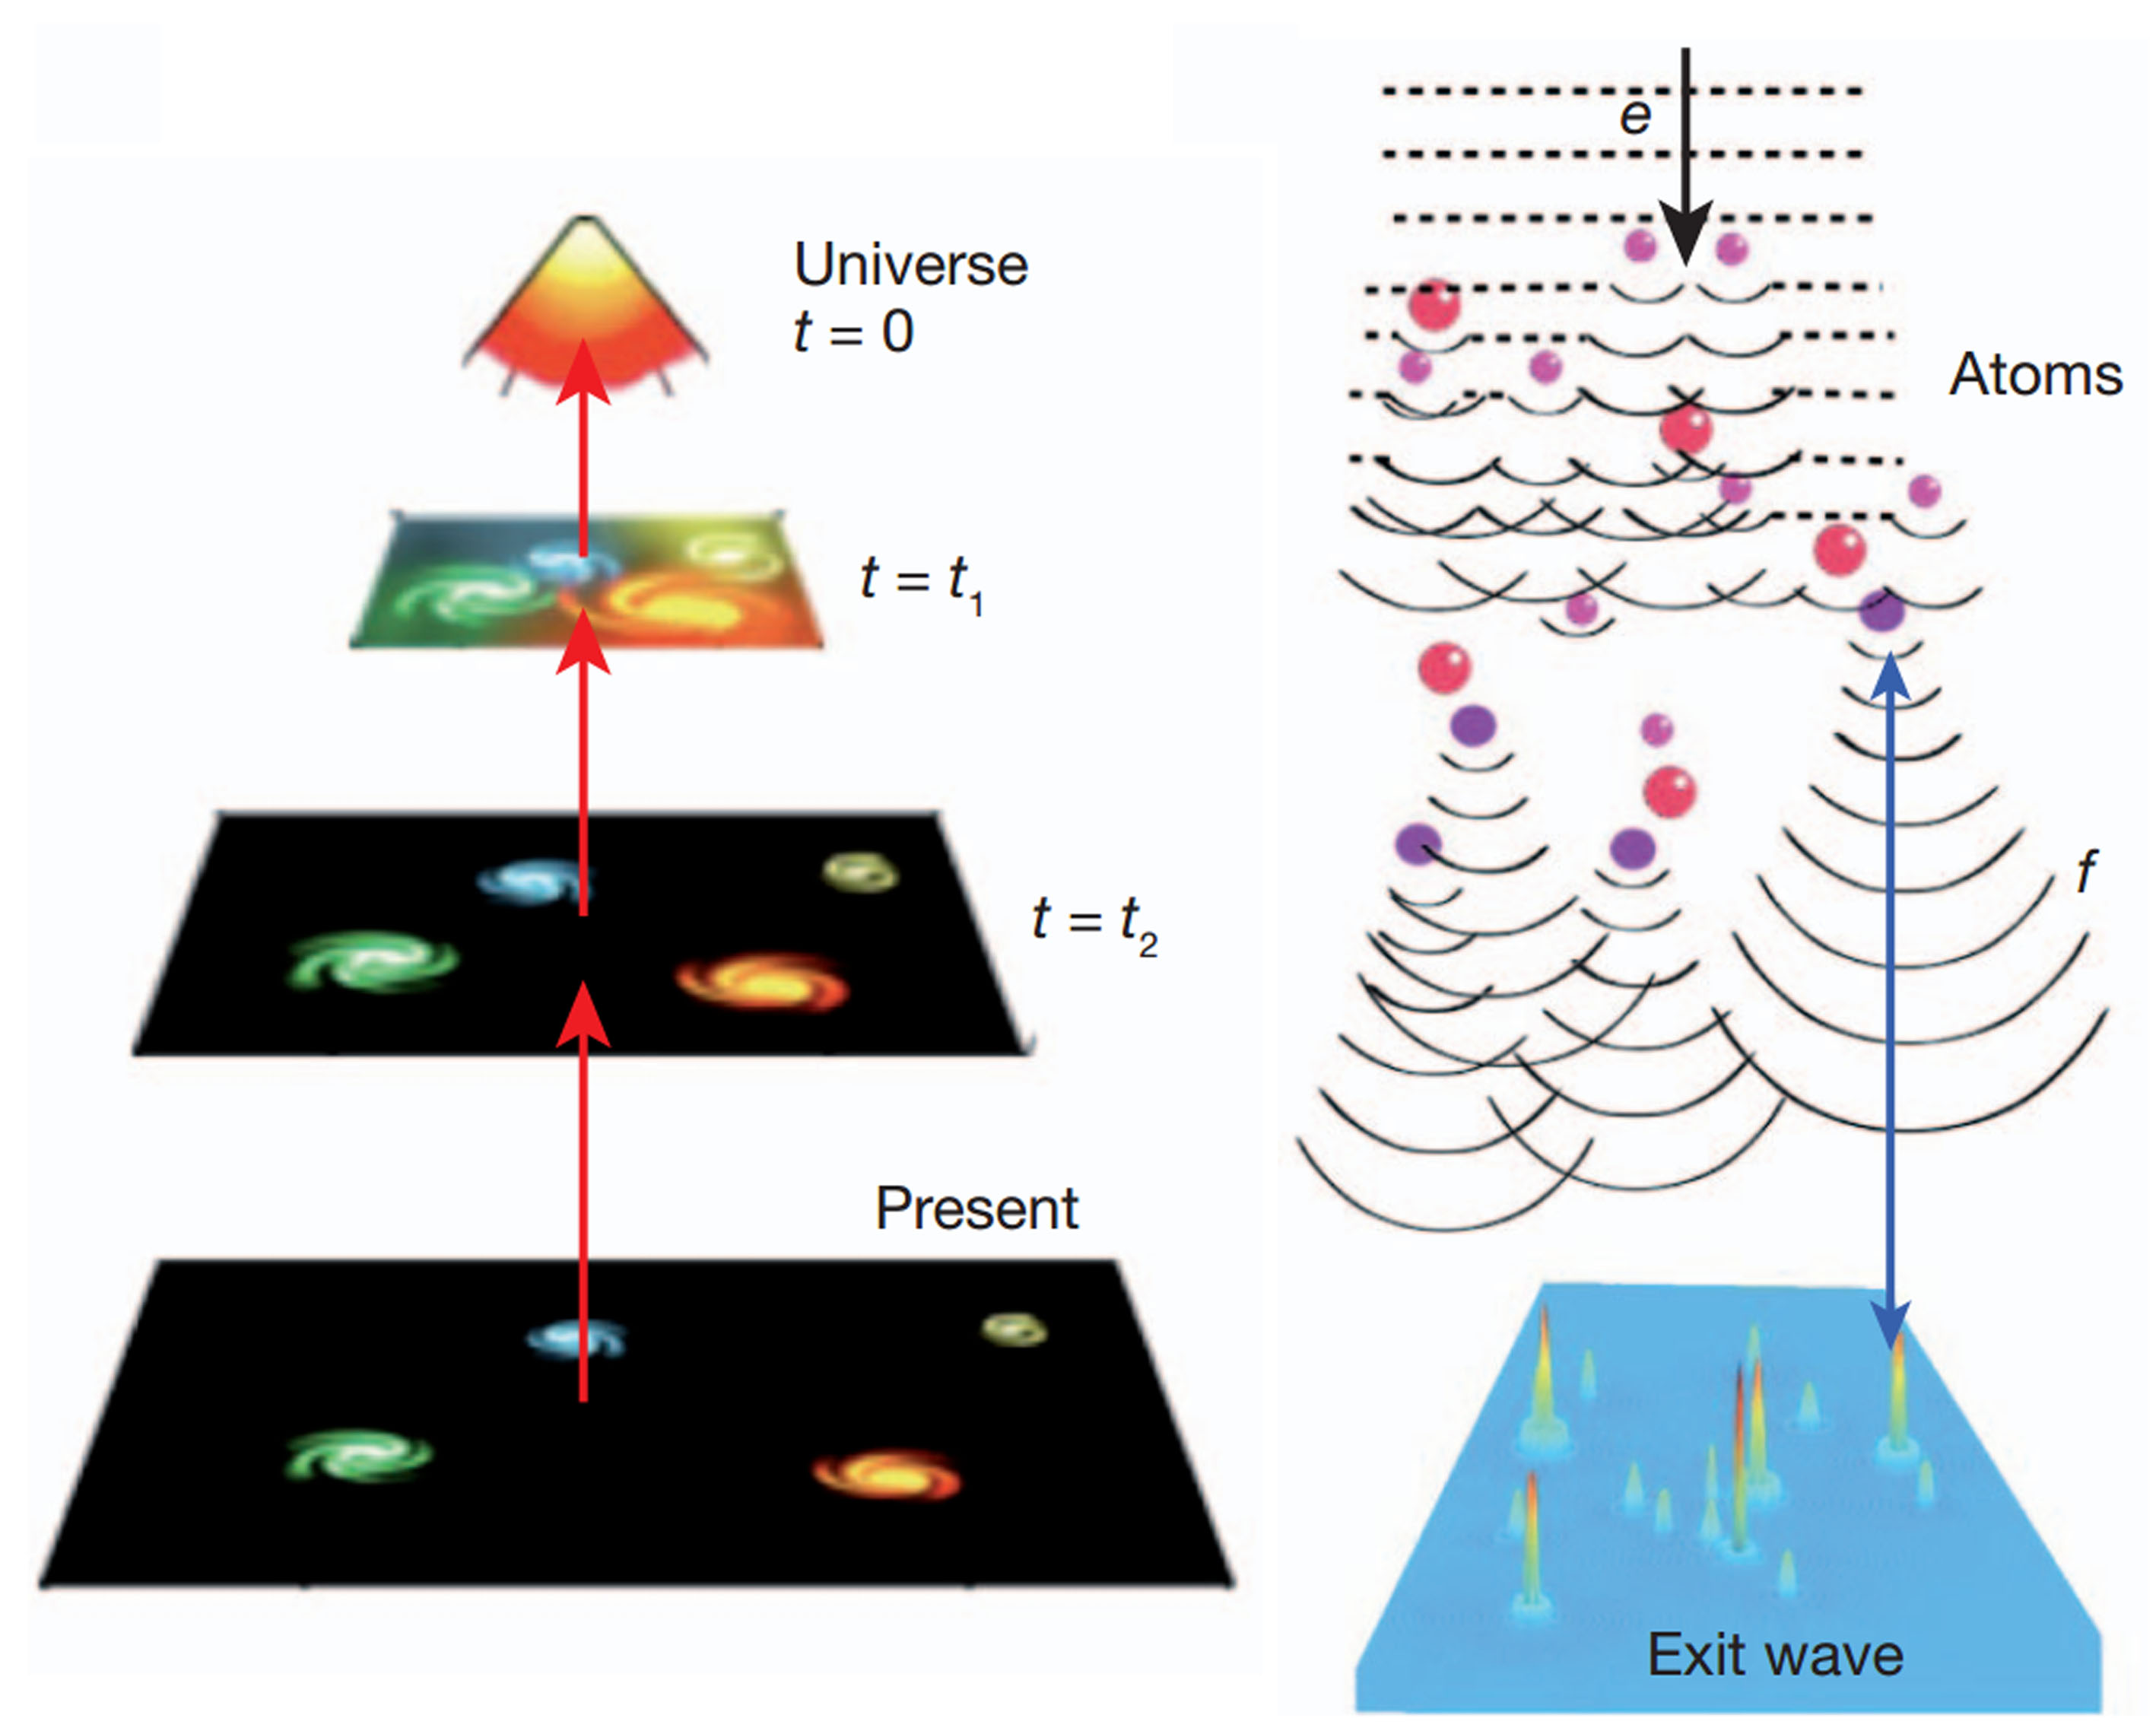
\includegraphics[width=0.8\textwidth]{../1.13/1_13}
	\caption{“Big Bang”三维重构原理示意图$^{[38]}$}\label{fig:113}
\end{figure}


在透射电子显微镜中,电子在离开原子后的自由传播过程可以由菲涅尔(Fresnel)传播表示:
\begin{equation}
\psi_e(\boldsymbol{r},z)=\psi(\boldsymbol{r})\otimes p(\boldsymbol{r,z}) = 1+iV_p(\boldsymbol{r})\otimes p(\boldsymbol{r},z)
\end{equation}
其傅里叶变换形式为:
\begin{equation}
\psi_d(\boldsymbol{g})=\delta(\boldsymbol{g})+f^{el}(\boldsymbol{g})\exp\left(i\left(\pi/2+\pi \lambda g^2f\right)\right)
\end{equation}
电子波在离开原子位置(欠焦量为“0”)后至欠焦量为“$f$”时,电子波相位的变化为:
\begin{equation}
\phi -\phi_0 = \pi \lambda g^2 f
\end{equation}
此式可变形为:
\begin{equation}
\pi \lambda g^2 = \frac{1}{f}(\phi-\phi_0)
\end{equation}
公式(1.66)可与公式(1.62)相比拟,$\pi \lambda g^2$ 称为“相位速度”,其中 $\lambda$ 是电子波长,$\boldsymbol{g}$ 是倒易空间矢量,相位 $\phi_0$ 在弱相位物近似中为 $\pi/2$。


在 TEM 中,出射面波函数重构和全息摄影技术都可以得到样品下表面的波函数~\cite{Ming2018,Ishizuka2013,Allen2004,Haigh2013,Morgan2011,Thust1996,OpdeBeeck1996,Zandbergen1996,Coene1992,Coene1996},由此可以实现电子波相位的测量。这使得欠焦量 $f$ 成为公式(1.66)中唯一的未知量,可以通过“相位速度”与相位的测量求出波函数所在平面相对于原子位置的欠焦量。测量步骤如图 1.16 所示,首先对重构得到的波函数通过三次样条插值进行二次采样,提高测量的精度。然后寻找出所有原子柱的位置,用软掩模将原子柱的波函数套选以供单独分析。之后扣除原子柱波函数的振幅和相位的背底,对其傅里叶频谱进行旋转平均。最后在频域中测量欠焦量 $f$。

通过测量每个原子的欠焦量,可以确定原子在 $z$ 方向上的相对位置,即重构了样品表面的原子的三维空间位置。

\begin{figure}[H]
	\vspace{\baselineskip}
	\centering
	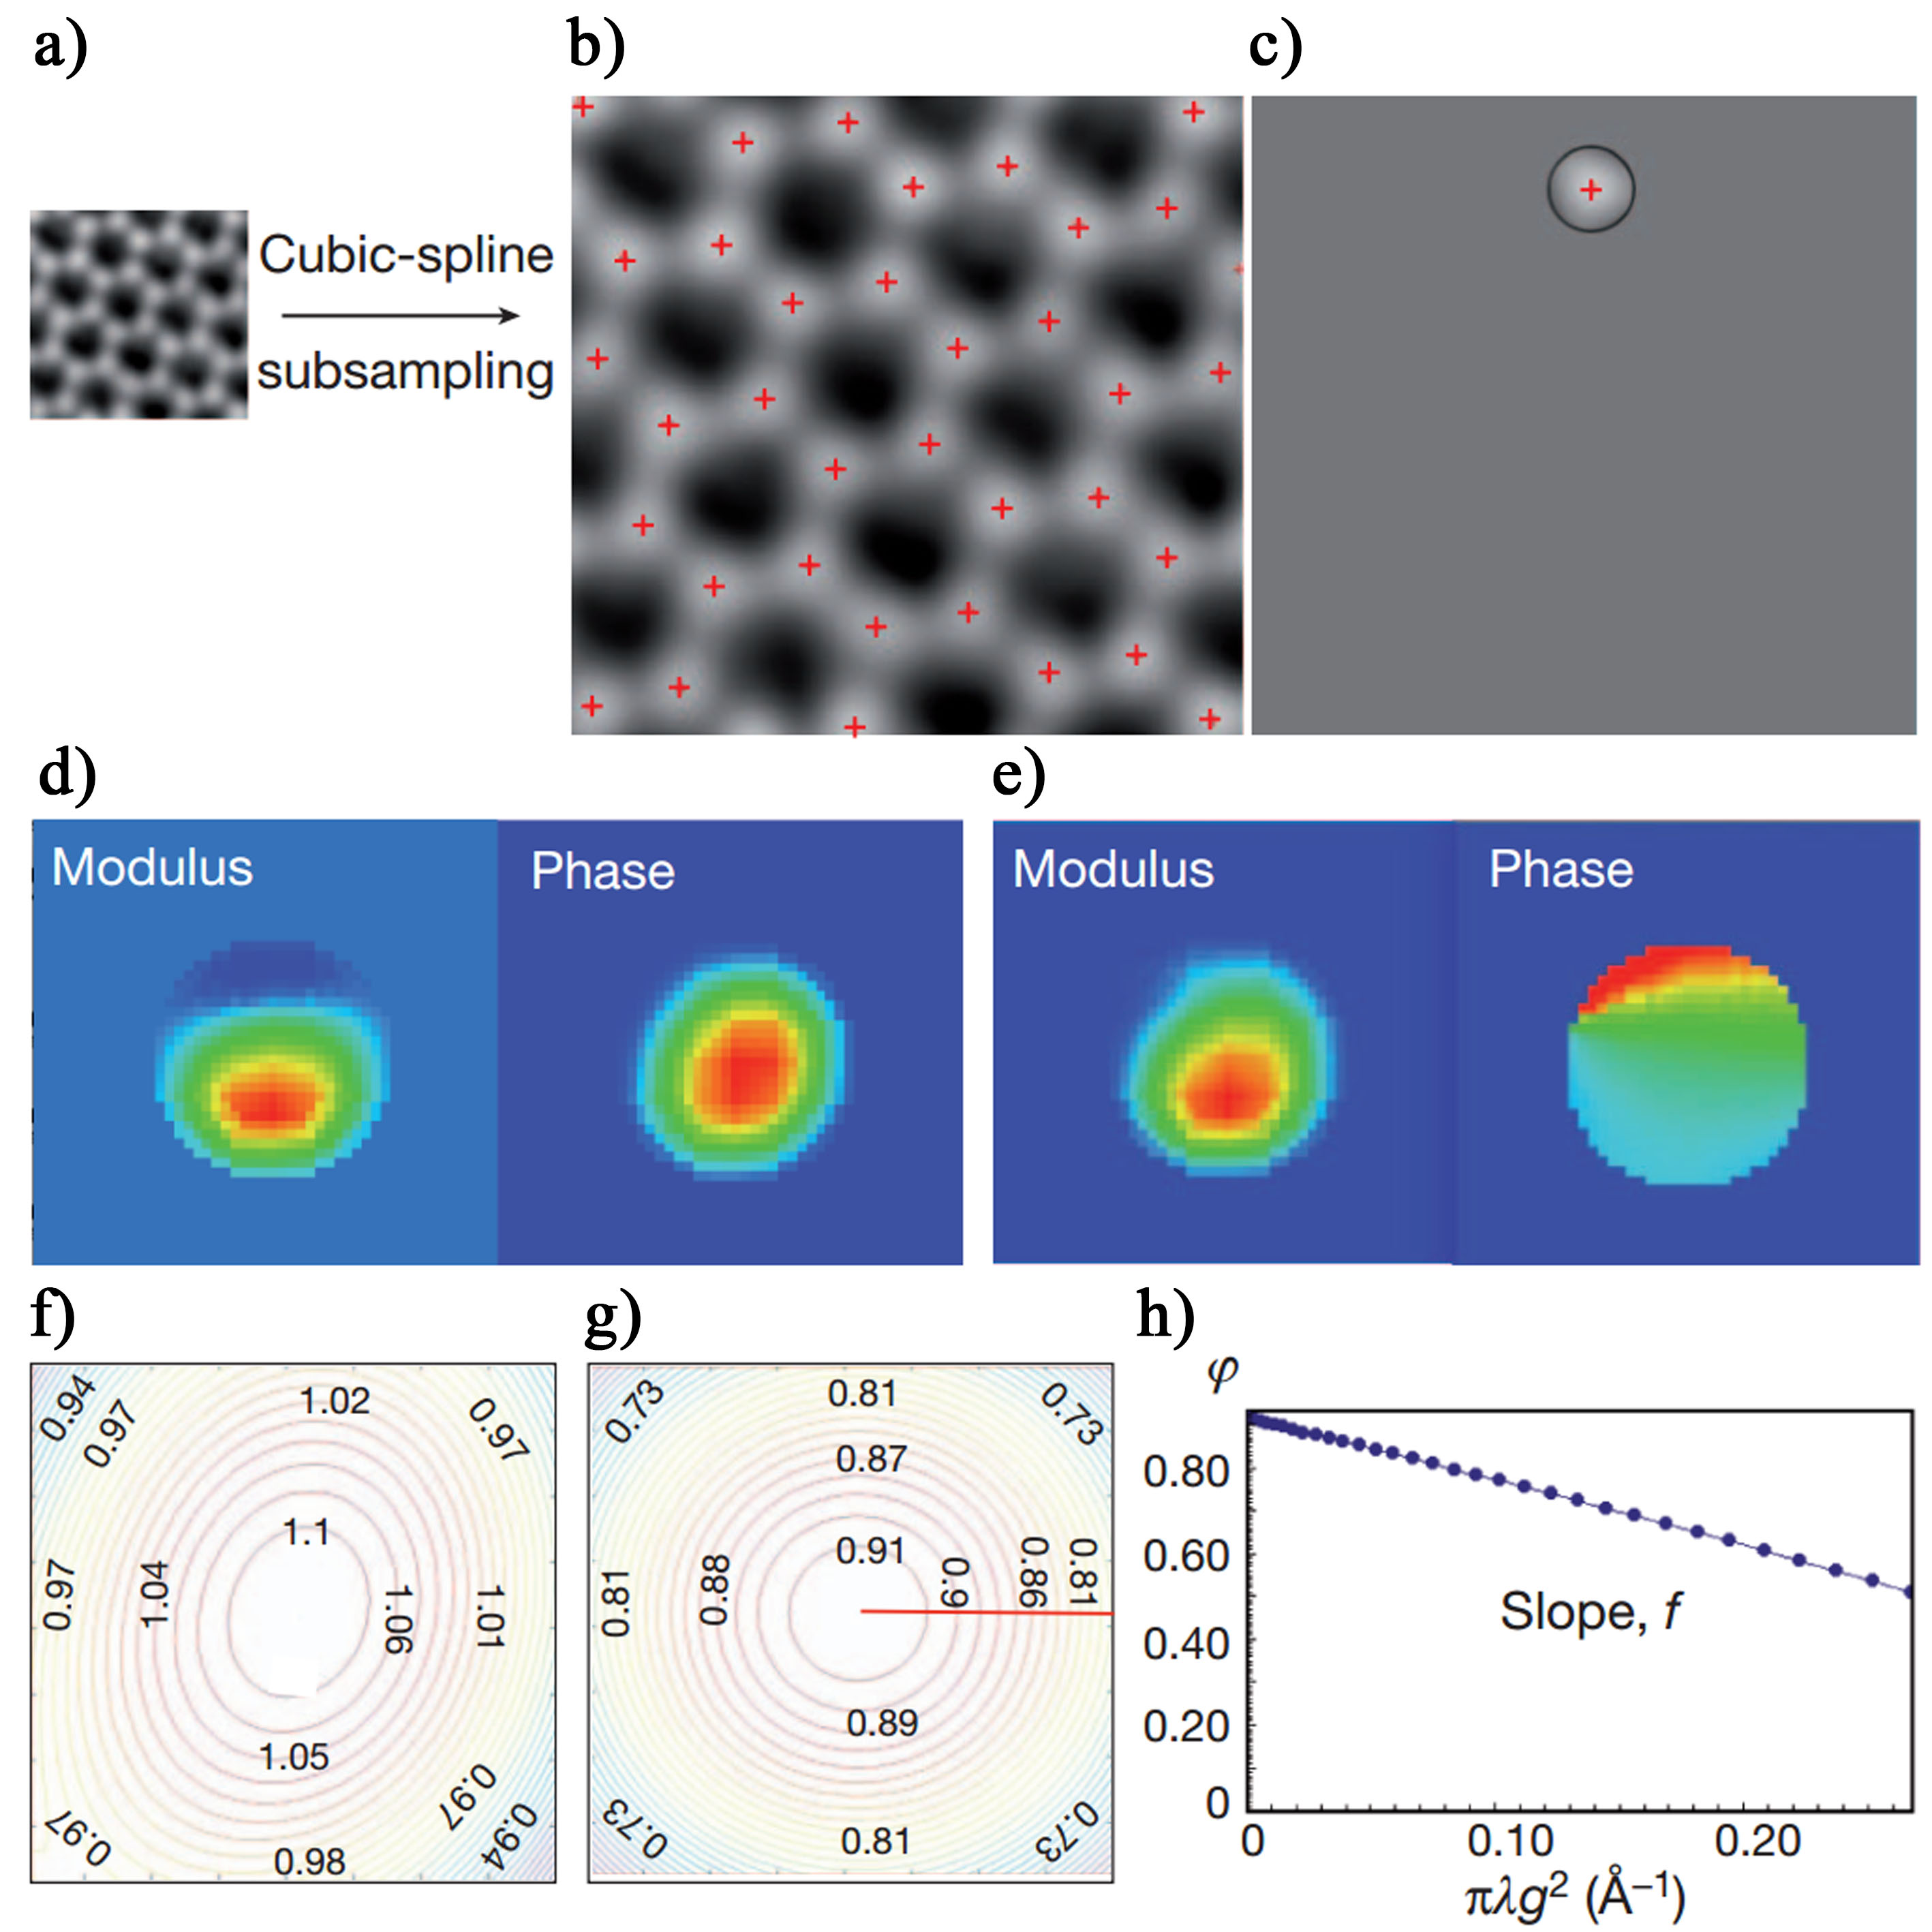
\includegraphics[width=0.61\textwidth]{../1.14/1_14}
	\caption{“Big Bang”三维重构流程图$^{[38]}$}\label{fig:114}
\end{figure}

\subsection{三维全息}
国立清华大学的 F.R. Chen 教授等通过多年的理论与实验研究,在 2016 年提出了三维全息(three-dimensional holography)的重构方法~\cite{ChenFR2017,ChenFR2016}。该方法基于通道理论(channeling theory),通过分析原子柱正下方的电子波的振幅与相位来确定该原子柱的原子个数和高度~\cite{ChenFR2015,WangA2012,WangA2010}。

\begin{figure}[htbp]
	\vspace{\baselineskip}
	\centering
	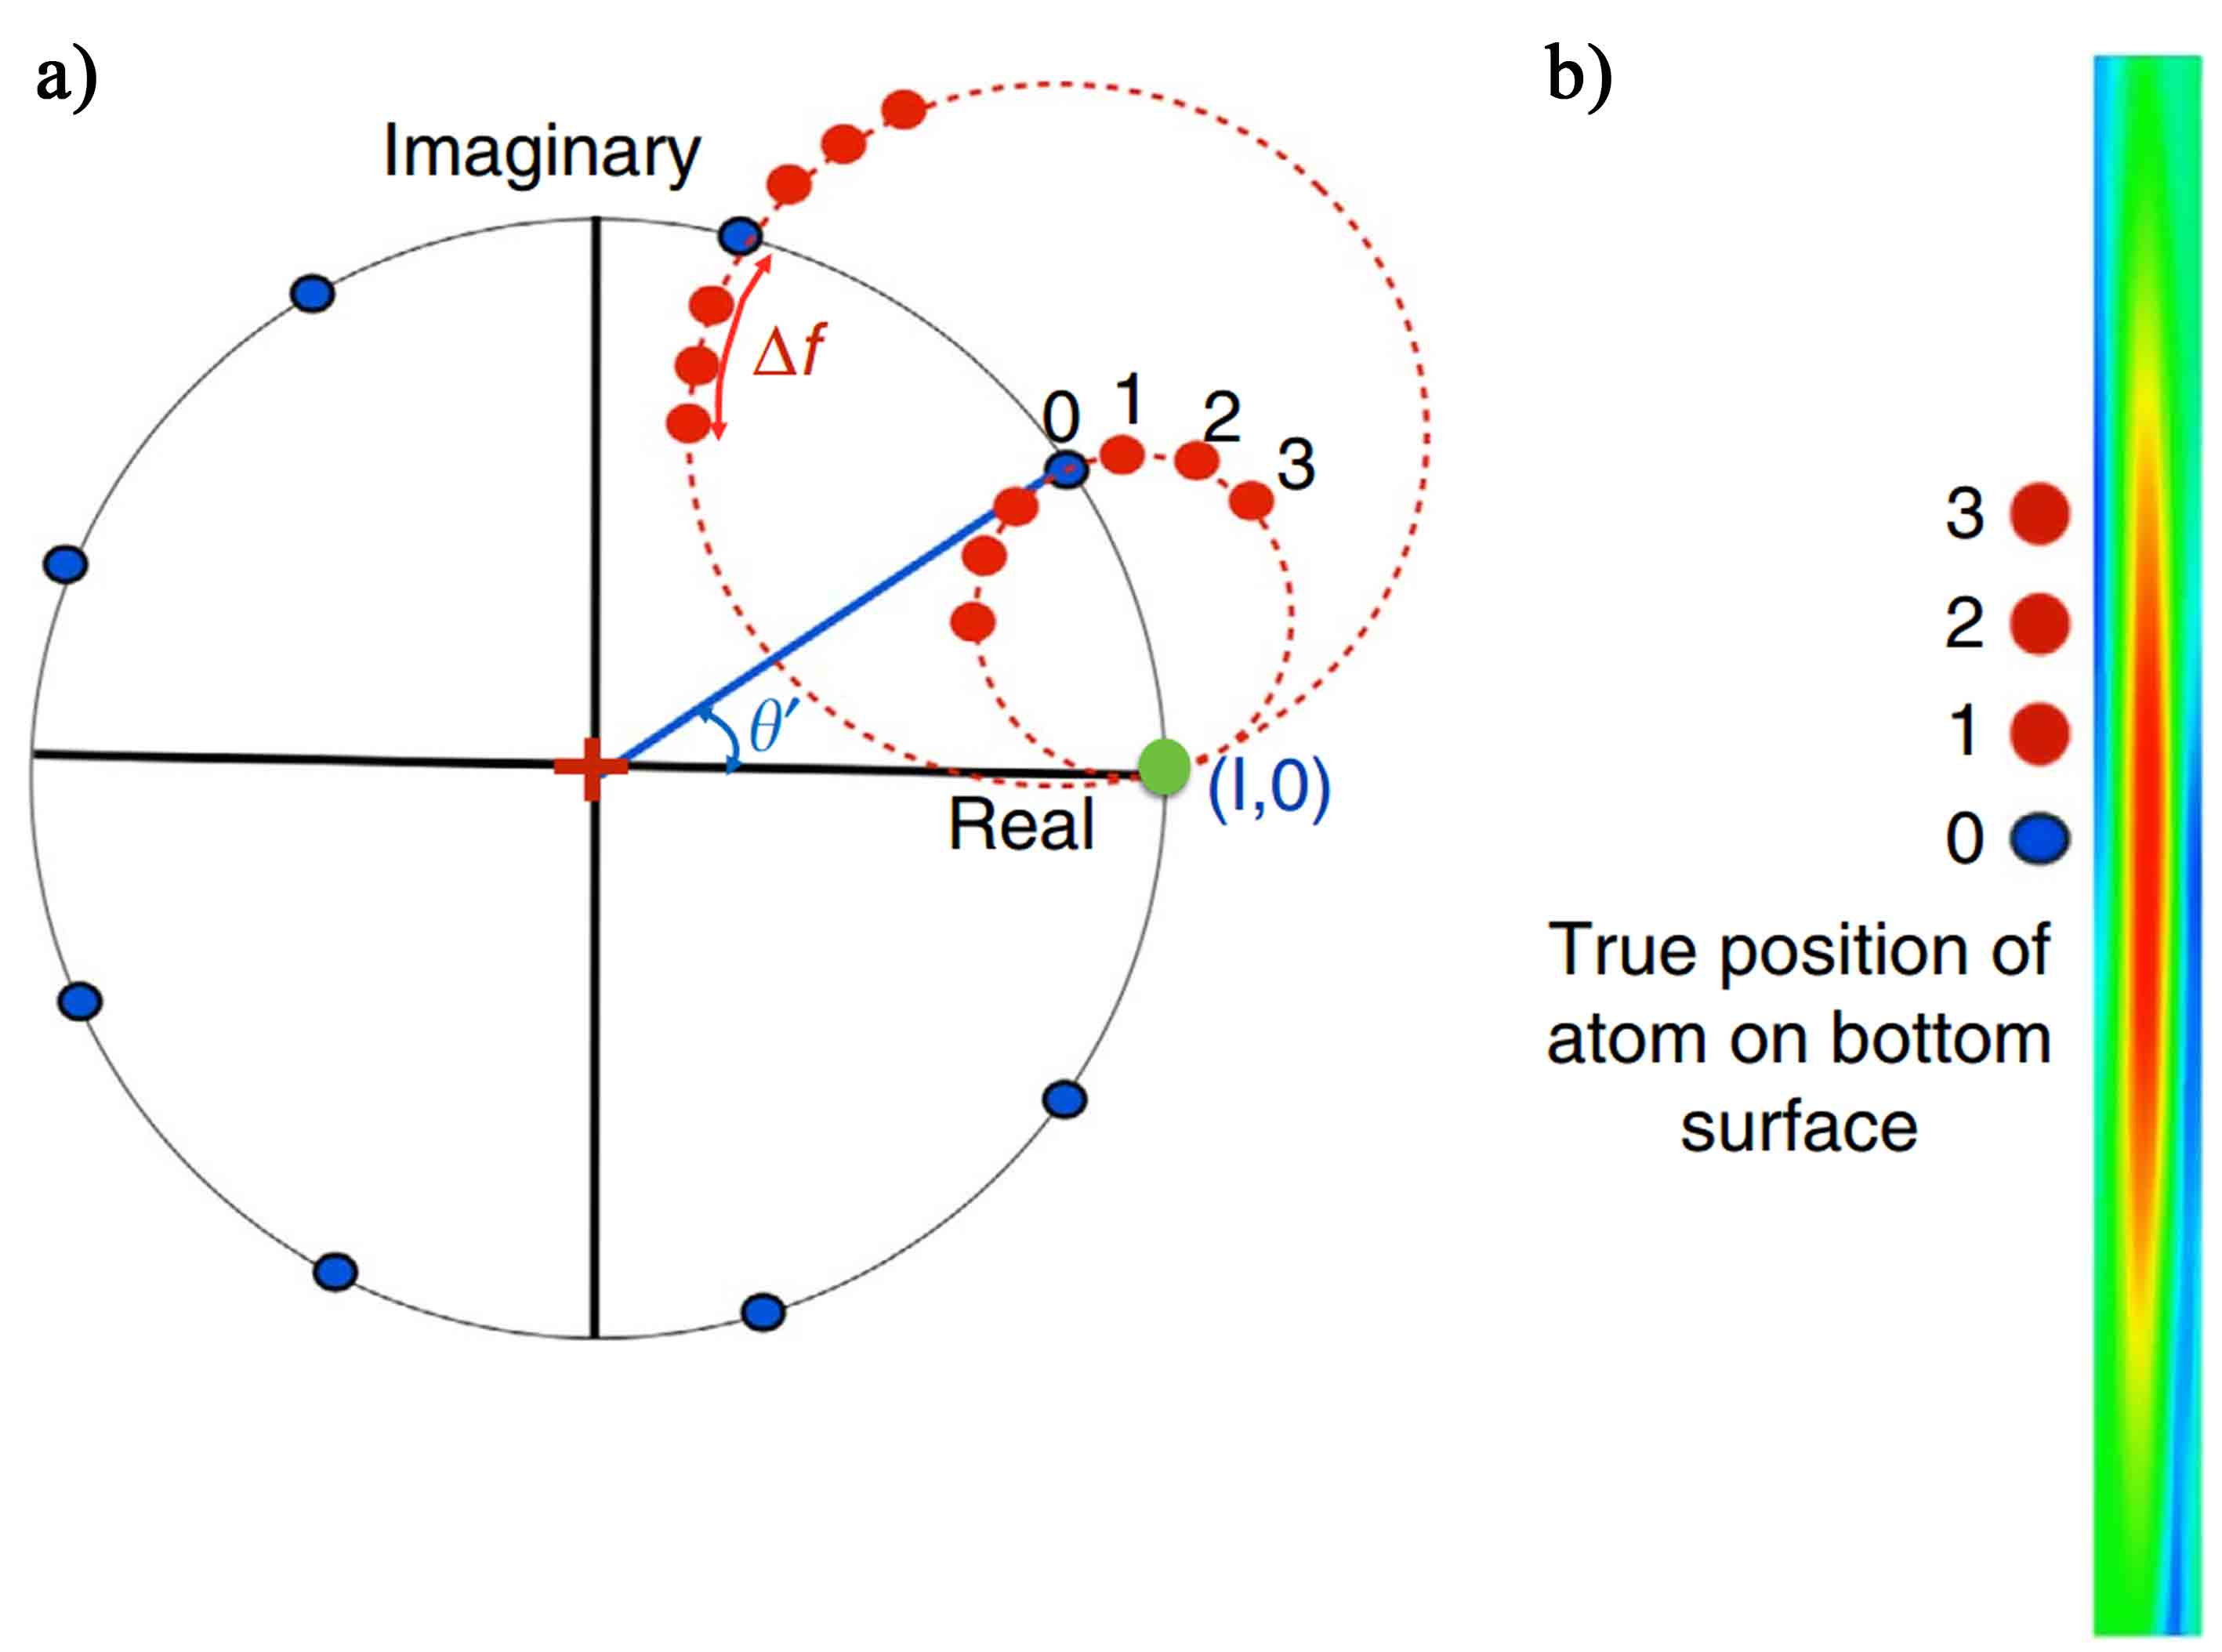
\includegraphics[width=0.8\textwidth]{../1.15/1_15}
	\caption{原子柱下表面波函数阿尔冈图和传播强度$^{[36]}$}\label{fig:115}
	\song\tuzhu{a) 阿尔冈图;b) 传播强度}
\end{figure}

通道理论认为,当晶体取向处于正带轴时,电子在孤立原子柱的下表面出射波函数可以由最低束缚态 s-state 表示:
\begin{equation}
\psi(\boldsymbol{r},z)=1+c_s\phi_s(\boldsymbol{r}-\boldsymbol{\beta})\left[\exp\left(-i\pi\frac{E_s}{E_0}kz\right)-1\right]
\end{equation}
其中 $\boldsymbol{r}$ 是垂直于电子束的二维平面矢量,$\boldsymbol{\beta}$ 是原子柱的位置,$E_0$ 是入射电子束能量,$k$ 是波矢,$z$ 是厚度。$E_s$ 是 s-state 方程 $\phi_s (\boldsymbol{r}-\boldsymbol{\beta})$ 的本征能量。
进一步推导可得电子波的实部与虚部分别为:
\begin{equation}
Re\left(\psi(\boldsymbol{r},z)-1\right)=-2c_s\sin^2\left(-\pi\frac{2E_s}{2E_0}z\right)\phi_s(\boldsymbol{r})
\end{equation}
\begin{equation}
Im\left(\psi(\boldsymbol{r},z)-1\right)=-2c_s\sin\left(-\pi\frac{2E_s}{2E_0}z\right)\cos\left(-\pi\frac{2E_s}{2E_0}z\right)\phi_s(\boldsymbol{r})
\end{equation}
不同原子个数的原子柱下表面的出射波函数在阿尔冈图(图 1.17)上分布在一个 mass-circle 上,即图中黑线所代表的圆。原子柱的厚度体现于波函数数值与入射波(1,0)点的夹角 $\theta^{\prime}$,原子柱的厚度增加,则该相位角也增加。对于不同的原子类型,每个原子引起的相位角增量不同。
进一步考虑欠焦量对波函数的影响,将传播因子 $p(\boldsymbol{g})=\exp(-i\pi \epsilon \lambda g^2 )$ 与波函数卷积得:
\begin{equation}
\psi(\boldsymbol{r},z)= 1+ c_s\frac{2\sqrt{2\pi} \alpha}{4\pi \alpha^2 + i\epsilon\lambda}\exp\left(-\frac{r^2}{4\alpha^2+i\frac{\epsilon\lambda}{\pi}}\right)\left[\exp\left(-i\pi\frac{E_s}{E_0}kz\right)-1\right]
\end{equation}
波函数随欠焦量在红色虚线圆 defocus-circle 上变化。图 1.17b 表示原子柱处的波函数在 $z$ 方向上传播时的强度变化。零欠焦的波函数具有最大的强度,且此时其数值与  mass-circle重合。

通过对电子波函数的传播,根据零欠焦模值最大的特点可以确定原子柱的欠焦量,并分析出 mass-circle,从而重构出所有原子柱的原子个数和位置。



\subsection{单张高分辨 TEM 图像三维重构}
2014 年,西安交通大学的 C.L. Jia 等提出了一种基于单张高分辨透射电镜原子像的三维重构方法,并成功重构了 MgO 样品的表面原子分布形貌~\cite{Jia2014}。

C.L. Jia 等使用了负球差成像~\cite{Jia2006,Jia2004,Urban2009,Jia2003,Jia1999}(negative spherical aberration imaging,NCSI)技术,在球差电镜中拍摄到了新鲜解理的 MgO 高分辨透射电镜原子像。他们认为,图像的强度不仅仅包含各原子柱的成分信息,更包含了原子柱在 $z$ 方向上的相对位置信息。所以,他们提出了一种基于像模拟的迭代优化程序来精确地分析图像中包含的材料的三维信息。程序的第一阶段是测量实验中的全局参数,比如样品的平均厚度、样品倾转、有效吸收常数、电镜的像差等。第二阶段是优化原子柱的位置和原子的占位,并且,第一阶段所测的参数也会在此阶段被进一步优化。原子柱优化的标准是比较局部原子柱的模拟和实验高分辨透射电镜图像的绝对强度,以期将原子柱强度分布的均方差降低到最小。

\begin{figure}[htbp]
	\vspace{\baselineskip}
	\centering
	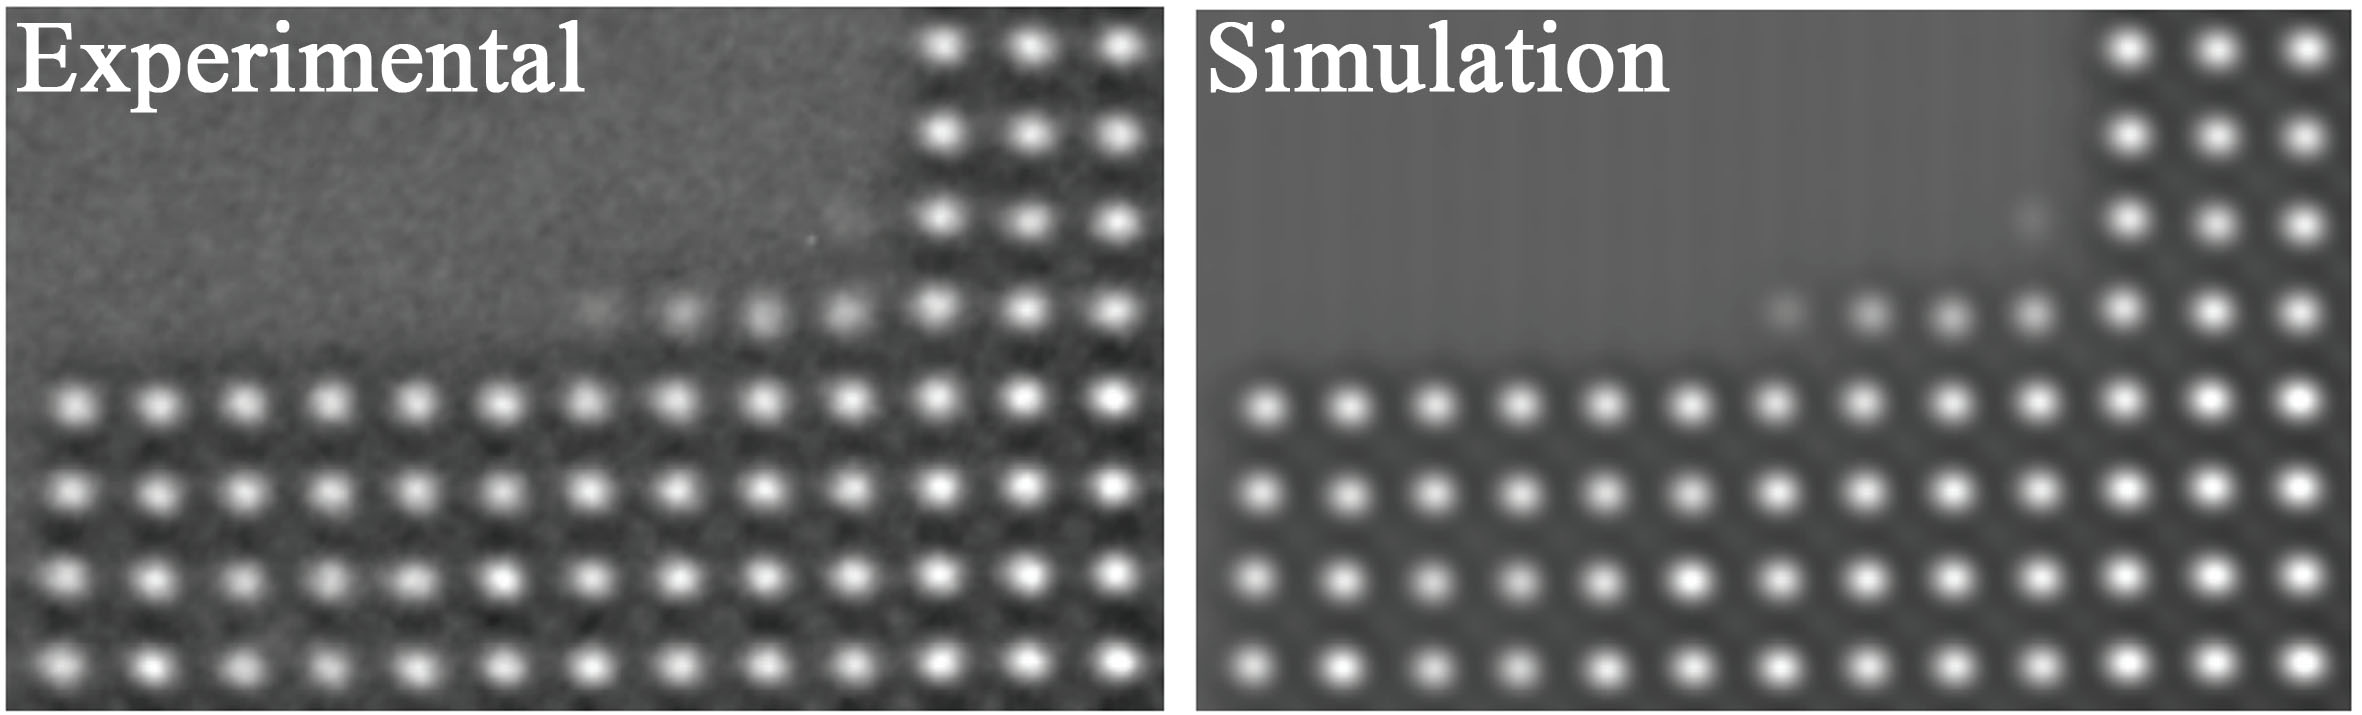
\includegraphics[width=0.8\textwidth]{../1.16/1_16}
	\caption{实验像与重构的模拟像$^{[37]}$}\label{fig:116}
\end{figure}

\section{本论文的主要研究内容}
本论文的研究着眼于实际 TEM 中三维重构技术存在的问题,通过改进或发展新的理论和方法,使三维重构技术在材料研究中获得更广泛的应用和更精确的重构结果。本论文主要研究了三个方面的内容:



1. 一般情况下,3DET 实验中总是存在缺失锥现象,在一般的 TEM 样品的重构中引起特别严重的假象。为了抑制这种假象,恢复缺少的信息,本文在第二章中开发了一种 ART 型的神经网络 3DET 算法。该算法不同于现存的抑制缺失锥假象的方法,它不引入任何先验知识来约束重构过程,而是利用高维度的神经网络实现对低维度的样品和实验数据的有效重构和信息恢复。所以,该方法除了能够有效抑制缺失锥假象之外,还具有广泛的适用性和良好的抗噪音能力。

2. 当 STEM 的电子束斑的横向分辨率达到埃量级及以下时,其纵向景深也会减小至纳米量级。此时,HAADF-STEM 像将不再是整个样品内部结构的线性投影,而会转变为样品内部某一深度的光学层析,不再符合倾转系列三维重构对线性投影的要求。本论文在第三章中通过理论模拟,探究了纳米尺度景深下原子分辨率三维重构的可行性。研究发现,当景深小于样品厚度时,三维重构技术只能正确重构样品中的局部区域。该区域的大小与入射电子束景深呈正相关,位置与入射束的欠焦量有关。另外,研究还发现实际正确重构的区域相对于电子束名义聚焦位置偏上,即存在提前聚焦现象,其偏离程度与样品内原子的原子序数、会聚角以及加速电压有关。当原子序数越大或会聚角越大时,其与名义聚焦位置偏离越大。

3. 原子分辨率三维重构新方法的发展还很不完善,现存的方法在应用上存在很大的局限性。本论文在第四章中提出了一种切实可行的通过单张高分辨 TEM 照片的定量分析重建一般晶体表面的原子分辨率三维重构技术。该技术采取全局匹配算法和自洽性验证方案,能够估计和定义三维重构的分辨率,并引入置信度来定量探究非晶对重构结果的影响。
